%\documentclass[12pt,manuscript]{aastex}
\documentclass[]{emulateapj}
\bibliographystyle{apj}
\usepackage{graphicx}
%\usepackage[suffix=]{epstopdf}
\usepackage{color}
\usepackage{natbib}
\usepackage{amsmath}
%         Make Scientific Notation
\providecommand{\e}[1]{\ensuremath{\times 10^{#1}}}
\usepackage{url} 

\shortauthors{Davenport et al.}
\shorttitle{2MASS Variability}

\begin{document}
 
\title{Periodic Variability from the 2MASS Calibration Scans}


\author{James R. A. Davenport\altaffilmark{1,2},
Andrew C. Becker\altaffilmark{2},
Peter Plavchan\altaffilmark{3},
Roc Cutri\altaffilmark{3}}

 
\altaffiltext{1}{Corresponding author: jrad@astro.washington.edu}
\altaffiltext{2}{Department of Astronomy, University of Washington, Box 351580, Seattle, WA 98195}
\altaffiltext{3}{Infrared Processing and Analysis Center, California Institute of Technology, Pasadena, CA 91125, USA}



\begin{abstract}

We report on a systematic search through the 2MASS Calibration Point
Source Working Database for systems exhibiting periodic variability.
While the total areal coverage of the data is modest, the temporal
coverage is significant, with more than 100 million 3--band
photometric measurements of 113,030 point sources.  Our sample
represents the most complete compendium of periodic variability in the
near--infrared.  Our data mining efforts recovered {\bf XXX} periodic
systems, which include {\bf XXX} eclipsing binary systems and {\bf
  XXX} radial pulsators -- {\bf XXX} RR Lyrae Type ab, {\bf XXX} RR
Lyrae Type c, {\bf XXX} Cepheids, and one short--period $\delta$ Scuti
star.  Hysteresis in the color--color evolution of these pulsating
systems provides valuable insights into the underlying stellar
astrophysics.  Our search also recovered {\bf XXX} quasi--periodic
long--period variables, which vary on a characteristic timescale, but
whose lightcurves are not repeatable cycle to cycle.  We examine
particularly rich variable star fields including those in $\rho$
Ophiuchus, and in the Small and Large Magellanic Clouds.  We outline
principles for multi--band periodic variable star classification using
periods and multi--band amplitudes and skews.  This will prove to be a
benchmark reference sample until large area, near--IR time--domain
surveys become a reality.

%data comes from 2mass-calpswdb, have over 100 million photometric measurements, totaling light curves for 113,030 point objects. we have run supersmoother period folding, ala MACHO, on every light curve. By hand verification used to check. many are found periodic, XX binaries, YY radial pulsators. These include the best sampled light curves for an RR Lyr and Cepheid variables in the NIR, and provide an important benchmark for modeling of these stars. An additional ZZ quasi-periodic variable stars are found. we have also characterized the variability properties as functions of color, finding nearly all objects have ``grey'' variability, where the amplitude is independent of wavelength chosen.
\end{abstract}


\keywords{variability, surveys, NIR}


%%%%%%%%%%%%%%%%%%%%%%%%%
\section{Introduction}
Arguably the two greatest advancements in optical and infrared photometric surveys within the past two decades have been the advent of 1\% accurate multi-wavelength photometry for contiguous portions of the sky exceeding $\Omega\sim10^4$ deg$^2$ \citep[e.g.][]{2006AJ....131.1163S,2010AJ....140.1868W,2011ApJS..193...29A}, and time resolved surveys spanning days to years baselines \citep[e.g.][]{2007AJ....134..973I,2011AJ....142..190S}. As both the temporal and spatial domains are explored, new astrophysical phenomena are uncovered, while previously rare events are placed in a statistical context. Naturally, next generation surveys will exploit both of these domains simultaneously, producing deep multi-wavelength surveys with both unprecedented spatial and temporal coverage \citep{2002SPIE.4836..154K,2008arXiv0805.2366I}. In order to prepare for these future surveys, which will contain orders of magnitude larger numbers of variable sources, existing catalogs and databases provide valuable insights into the data complexity, and serve as testing grounds for identification and classification of phenomena. Such studies will precipitate the development of new techniques, which in turn may inform the targeting, cadence, and observing strategies of the future surveys \cite[e.g.][]{2012AJ....144....9O}.

%WISE will provide huge variability data in the mid IR for regions near the orbital poles. Many papers using NIR variability to study new physics. The VVV (VISTA variables in the V{\'{\i}}a L{\'a}ctea) survey in the bulge, DR1 just release \citep{vvv_dr1}

The Two Micron All Sky Survey \citep[2MASS;][]{2006AJ....131.1163S} imaged the full sky in three, simultaneously obtained, near-infrared (NIR) bands. Survey operations were conducted between 1997 and 2001, using a northern and southern telescope. Photometric calibration for 2MASS was accomplished using repeated observations of 35 selected fields, which were spaced across the sky \citep{2000AJ....120.3340N}. An additional 5 tiles were imaged around the Large and Small Magellanic Clouds during the last year of operation. Each calibration field covered an area of approximately 8\farcm5 (RA) $\times 1^\circ$ (Dec). The 35 standard calibration fields were scanned ranging between 562 and 3,692 times over the 4 year period, yielding some of the most densely sampled and well--calibrated NIR light curves yet produced. The placement of these tiles is shown in Figure \ref{radec}, and they contain light curves for approximately 110,000 point source objects.  These data were released as part of the 2MASS Extended Mission \citep{Cutri-2massExtended}, and collectively define the 2MASS Calibration Point Source Working Database (Cal--PSWDB).

This unique dataset has been used for a handful of studies to date. 
\citet{2008ApJS..175..191P} characterized many of the details in analyzing this unique dataset for time domain studies. They also mined these data for periodic objects, finding 3 new M dwarf eclipsing binaries. 
\citet{2008ApJ...684L..37P} studied the 131 day periodic object, 2MASS J16271848--2429059, revealing a possible three-body YSO system. 
\citet{2009ApJ...698.1872S} utilized the images from multiple scans of calibration tile 90067 to produce a NIR color-magnitude diagram for the open cluster M67 that probed $\gtrsim$3 magnitudes deeper than the standard 2MASS point source catalog. 
\citet{2008MNRAS.386..416B} discovered and characterized a 2.6--day periodic M dwarf binary, 2MASS J01542930+0053266. This system was located in both the 2MASS calibration tile 90004, and the ``Stripe 82'' region of the Sloan Digital Sky Survey footprint, which yielded an 8-band light curve ($ugrizJHK_s$) for the binary. 
Using 16 of the calibration tiles that overlapped the SDSS footprint, \citet{2012ApJ...748...58D} produced some of the first constraints on the properties of M dwarf flares in red optical and NIR bandpasses. 


{\bf 
MENTION THESE TWO? 
(P. Plavchan 2012 submitted) an analysis of a 92 day periodic YSO. 
(J. Parks 2012 submitted) a detailed study of the $\rho$ Ophiuchus star forming region tile. 

ADD PARAGRAPH PROMPTING USE OF 2MASS AS CENSUS FOR VARIABLES -- TAKE IDEAS FROM PROPOSAL
}

In this paper we present a census of the periodic variable objects from the time--domain calibration data. The data and period-finding methodology are outlined in \S2. We describe the selection and classification of binary stars and radial pulsating objects in \S3. Quasi-periodic and other large amplitude variables that were recovered are discussed in \S4. We examine the general variability characteristics of point sources in the 2MASS calibration scans in \S5, and concluding remarks are given in \S6.



%%%%%%%%%%%%%%%%%%%%%%%%%
\vspace{.1in}

\section{Data}


\begin{figure*}[!t]
\centering
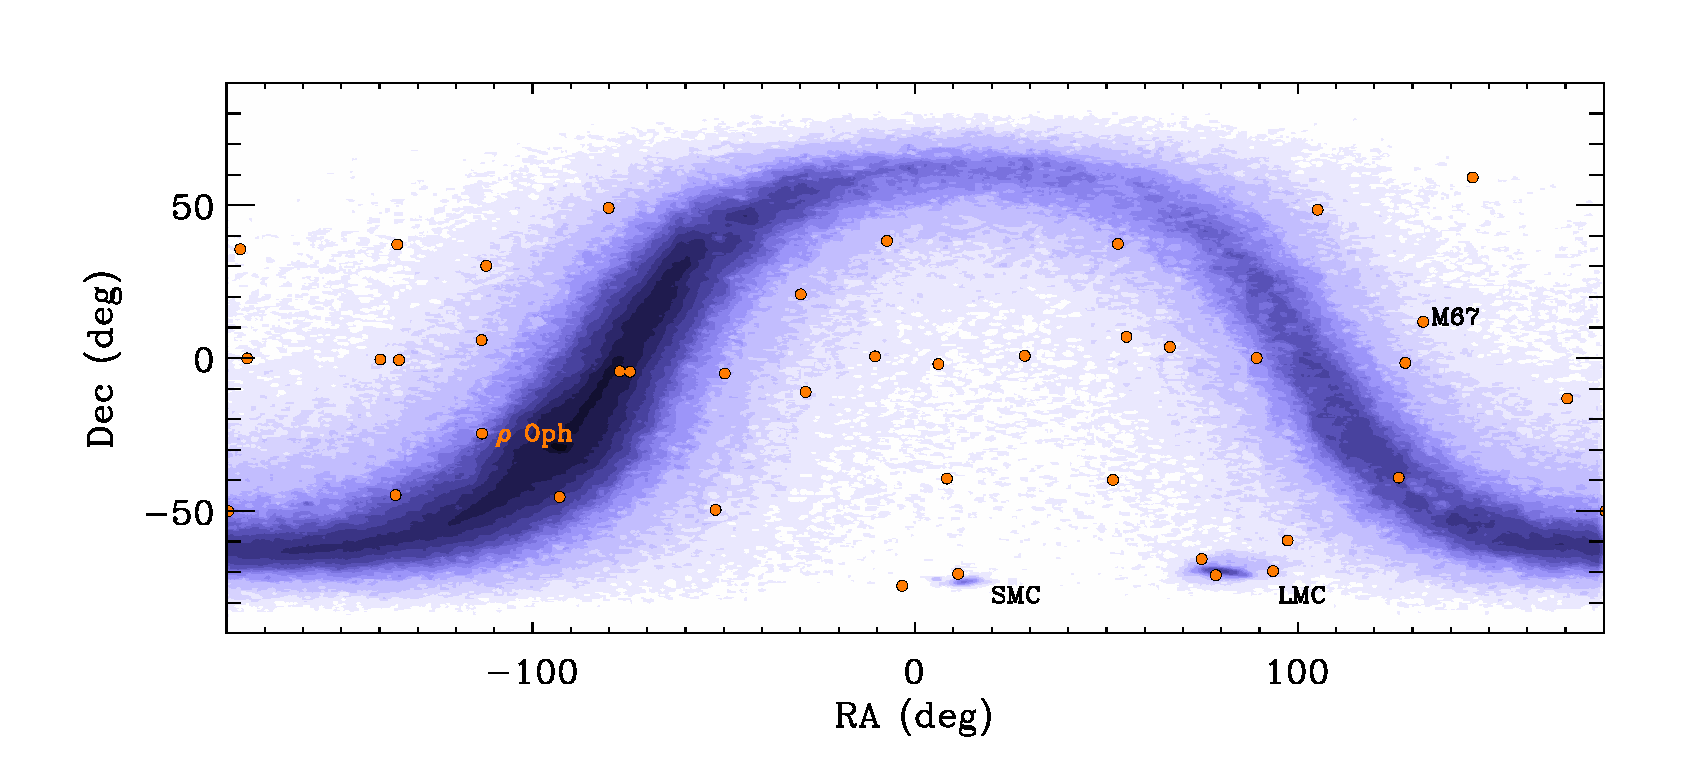
\includegraphics[width=7.0in]{new_plots/radec_psc}
\caption{Spatial distribution of the 40 Cal-PSWDB tiles (orange circles), with titles for a few notable tiles labeled. Background contours denote increasing density from a sample of 3 million randomly drawn point sources from the 2MASS point source catalog, and trace the Galactic plane, bulge, and the Large and Small Magellanic Clouds.}
\label{radec}
\end{figure*}

\vspace{.01in}



%\begin{figure*}[!t]
%\centering
%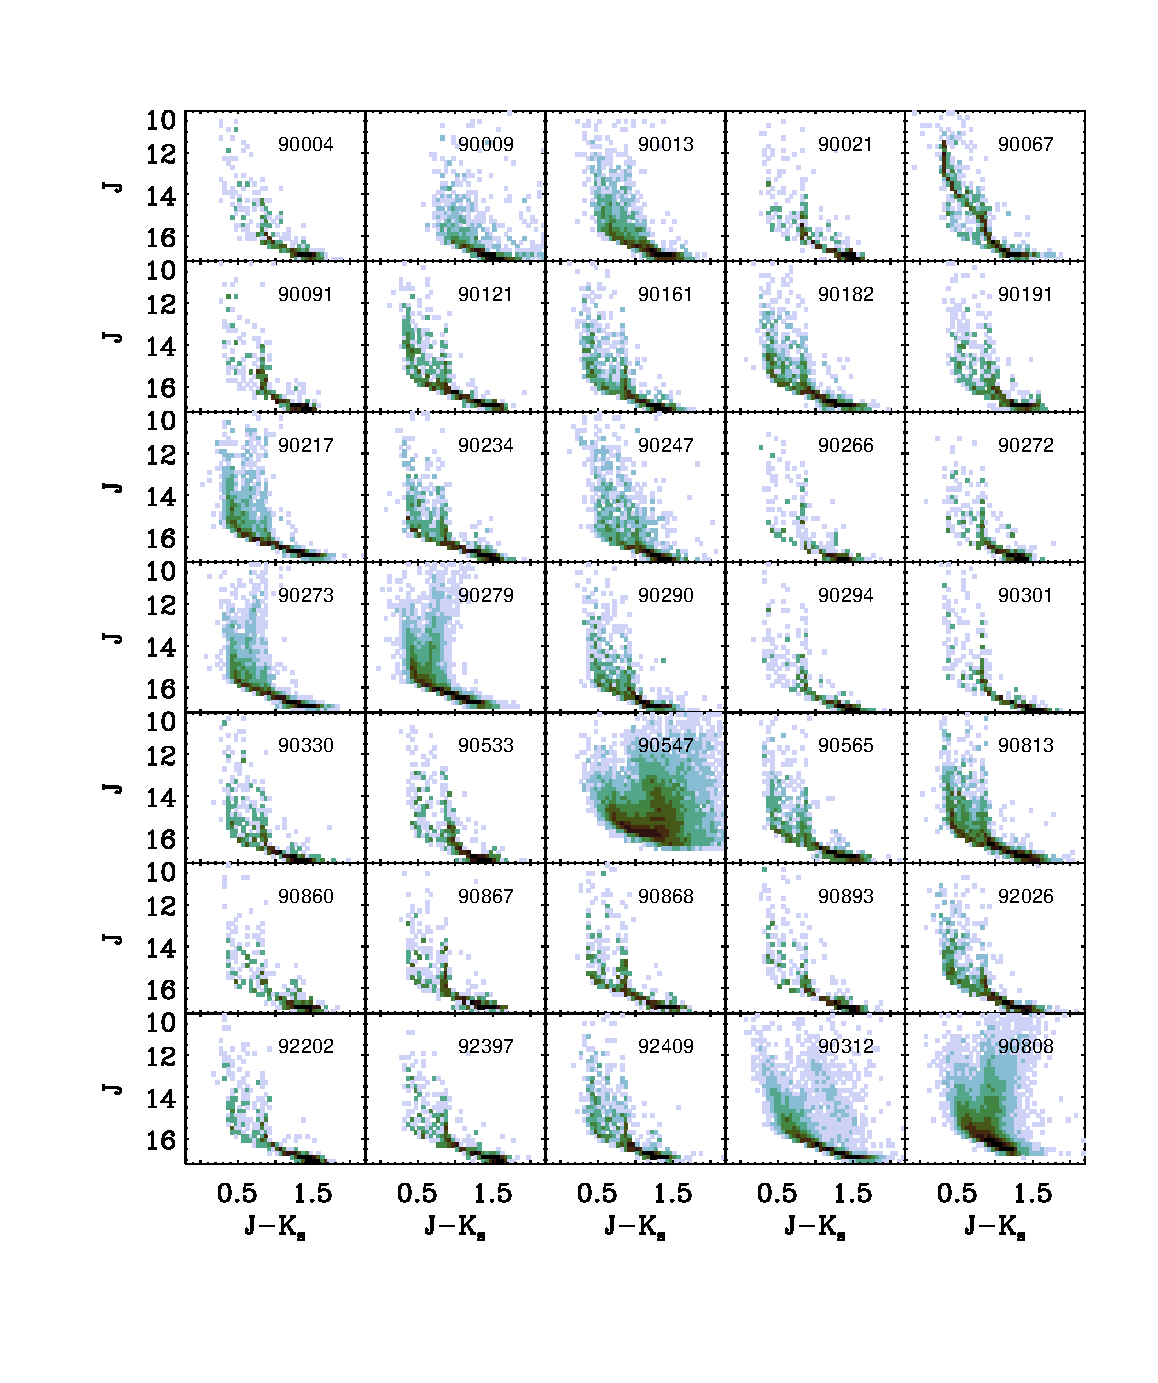
\includegraphics[width=7.0in]{new_plots/big_cmd1}
%\caption{color mag diagrams for the fields}
%\label{cmd1}
%\end{figure*}
%\clearpage
%
%\begin{figure*}[!t]
%\centering
%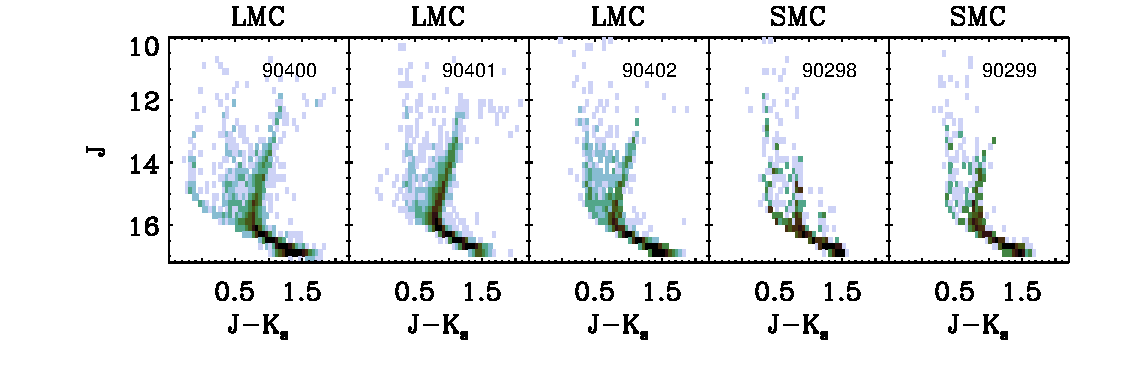
\includegraphics[width=7.0in]{new_plots/big_cmd2}
%\caption{color mag diagrams for the LMC/SMC fields}
%\label{cmd2}
%\end{figure*}


Each night during 2MASS survey operations, the telescopes observed one
of the calibration fields every hour (before 1997 October, two fields
were observed every 2 hours).  The three--channel cameras employed by
2MASS allowed for simultaneous imaging in the $J$ (1.25 $\mu$m), $H$
(1.65 $\mu$m) and $Ks$ (2.17 $\mu$m) passbands.  During each visit, six consecutive scans of the field were made in alternating declination directions in $\sim$10 minutes of elapsed real time. Each scan in the set of six was offset from the preceding one by $\sim$5" in R.A. to avoid systematic pixel effects. The calibration scans were observed using the same ``freeze-frame'' observing strategy used for the main survey, which yielded a net 7.8 s exposure on the sky per scan. {\bf IS THIS TRUE} The combination of the 6 scans yielded a single ``observation'' for the purposes of this study.  Over the course of the 2MASS survey, between 562 and 3692 independent observations were made of each of the 35 calibration fields. In the final year of the survey, 5 additional fields the Small and Large Magellanic Clouds were repeatedly observed, and are also included in this study.  Table 1 presents a list of these fields and their aggregate properties.

Lots of testing, characterization of the Cal-PSWDB done in \citep{plavchanphd,plavchan2008a}

The raw imaging data from each scan of a 2MASS calibration field were reduced using the same automated data processing system used to process the survey observation data \footnote{http://www.ipac.caltech.edu/2mass/releases/allsky/doc/explsup.html}. The reduction process detected and extracted source positions and photometry for all objects in the images from each scan. Measurements of the standard stars in each field were used to determine the nightly photometric zero-point solutions as a function of time, and seasonal atmospheric coefficients. All source extractions from all scans were loaded into the 2MASS Calibration Point Source Working Database (Cal-PSWDB). This database contains over 196 million source extractions derived from 74,772 scans of the 35 calibration plus 5 Magellanic Cloud fields. 

We acquired the entirety of the Cal-PSWDB and LMC/SMC Cal-PSWDB
through a bulk catalog download, and ingested all data into a MySQL
database.  In these original data, the {\tt gcntr} field was used as a
unique identifier for all the merged point--source detections,
i.e. all sources with the same {\tt gcntr} should be associated with
the same astrophysical object.  However, the distributions of
astrometric centroids for a significant number of these objects
appeared multi--model, indicating an insufficient job of
catalog--level deblending.  For this reason, we performed a wholesale
reanalysis of all of the source positions, clustering them into a
final set of 113,030 ``objects'' using the {\tt OPTICS} algorithm
\cite{optics}.  These objects have on average smaller RMS centroid
uncertainties and longer lightcurves, indicating that {\tt OPTICS}
both performed a better job of deblending and at associating epochs
together.  For objects brighter than $J = 16$, the median number of
$J$--band measurements increased from 432 to 671, while the median RMS
of the astrometric centroids modestly decreased to 0.10'' from 0.11''
(when including objects fainter than $J=16$, the median astrometric
RMS decreased to 0.28'' from 0.41'').  Bulk lightcurve metrics were
calculated using only data with photometric quality flags ``A''
through ``C'', effectively limiting us to S/N $>$ 5, and corrected
photometric uncertainties smaller than 0.22 magnitudes.







%%%%%%%%%%%%%%%%%%%%%%%%%
\section{Periodic Variables}

To search for periodically variable objects, we used the {\tt
  Supersmoother} algorithm that has been used in many previous
astronomical datamining applications
\citep[e.g.][]{2011ApJ...731...17B}.  Data from each of the three
passbands were smoothed independently, resulting in 3 period estimates
per object.

%each light curve was processed with Supersmoother
%objects with periods in at least 2 bands that were not obviously aliases were grabbed (about 2000 objects)
%each light curve was examined by eye, about 250 were bona fide good periodic objects

\subsection{Selection Criteria}
To select objects likely to be periodic, we examined the periods
returned in each of the three passbands.  We applied two sets of
criteria based upon previous multi--band periodic variability
studies.  Because {\tt Supersmoother} will report periods even when
none are supported by the data, all stars in each candidate list were
visually inspected to verify the periodicity of the system, and to
classify the sources.

The first selection criterion looks purely at the standard deviation
of the period estimates, similar to the analysis of
\cite{2011ApJ...731...17B}.  Briefly, this requires that the standard
deviation of the period estimates, or of the period estimates
corrected for aliasing, are smaller than $10^{-4}$ of their average
value. This was done using all 3 periods, and as a looser cut, using
only two of the three periods, since the $K_S$--band data typically
have both lower signal--to--noise measurements and smaller lightcurve
amplitudes.  This cut yielded 2073 candidates, each of which were
folded at the reported periods and validated through visual
inspection.  In total 157 systems from this list were verified as
periodic systems.

As noted by \cite{2012AJ....144....9O}, this may present too stringent
of a cut for longer period systems.  Because such systems will have
gone through fewer oscillations in a given time window, their period
is likely to be more poorly constrained.  For this reason, we apply a
second criterion, which requires that the standard deviation of the
periods divided by their average {\it squared} is less than $10^{-5}
{\rm day}^{-1}$.  This set of cuts yielded 696 systems, of which 570
were new candidates (meaning it recovered 126/157 of the previous
objects).  XXX of these pass the human validation, and are included in
this publication.

\begin{center}
{\color{red} \line(1,0){250}}
\end{center}

things that SUPERSMOOTHER said were periodic in at least 2 bands we looked at, returned 2100 interesting objects. we searched all 2000 light curves of periodic things by eye to pick out the real ones. quite a few are noise. found correct periods by hand, trying folding objects at 1/2, 2, 2/3 etc. also folded at all periods determined for each band.  

we also put the objects in to 4 classification bins by hand: obvious binaries with distinct eclipses, objects with very RR Lyr looking saw-tooth light curves, and sinusoidals which could be either W UMa or RR Lyr (a/b?). we also noted quasi-periodic or long period objects whose periods were not well sampled enough to accurately determine. those could be things like Miras, etc. this recovered 160 binaries, 8 pulsators. 25 other things.


to quantitatively separate these things, need a more impartial method. Eclipsing binaries and pulsating variables can be separated and classified by fitting Fourier modes to the light curves \citep{pojmanski2002,nefs2012}.. we used similar methods as other authors, using the IDL FOURFIT package by Buie (online CITE/footnote).


the binary type separation has been well-explored, and we use previously established equations (CITE Becker? for example). this puts them in 3 categories, which had excellent agreement with our initial by-eye analysis. we recover XX detached, YY semi-detached objects. contact binaries are called W UMa type, have very sinusoidal light curves. these are difficult to distinguish from rr lyr. sometimes they have color variations, but sometimes not if the mass ratio is near 1.

the separation between binary stars and rr lyrae is more difficult. some types of RR Lyr look very similar to binaries, most especially RR Lyr type a (CHECK ON THIS).  to improve this, we need other types of Fourier cuts to quantify the asymmetry in the light curves. there is some previous work on this (\citep{aaas}?) but we found their cuts didn't make sense, possibly due to different fitting codes (?) or different wavelength(?). 

using our by-eye categorization for objects, 8 for sure pulsators, we explored many combinations of Fourier parameter space. a4/a2 had been suggested previously as a good space to search in \citep{asas}. b1 makes sense, it is the first component of cosine asymmetry from the sinusoidal shape. binaries with eccentricity near 0 should not have any strong b modes. 



To separate binaries from pulsators, we cut on:
\begin{equation}
b_1({\rm binary}) \ge  -0.13\left( \frac{a_4}{a_2} \right)- 0.3
\end{equation}

and different configurations of binaries can be determined using:
\begin{eqnarray}
a_4({\rm detached}) \ge & a_2(0.5 + a_2)\\
a_4({\rm contact}) \le & a_2(0.125 + a_2)
\end{eqnarray}

\begin{figure}[]
\centering
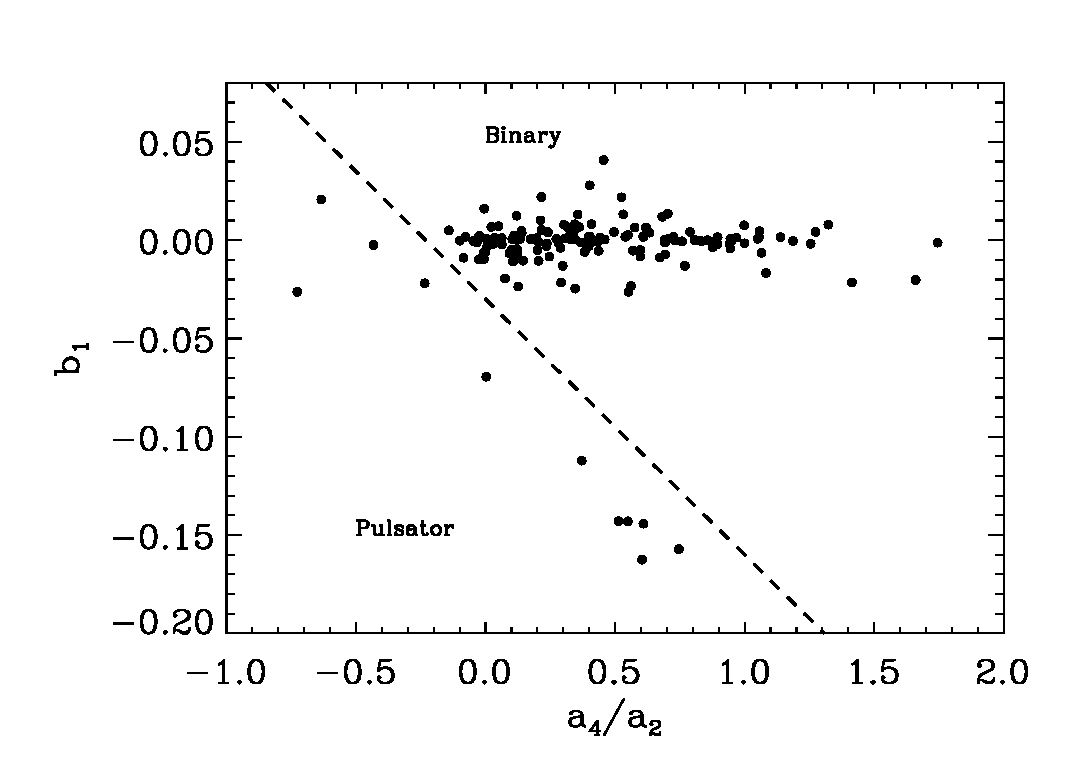
\includegraphics[width=3.5in]{new_plots/four_a42b1}
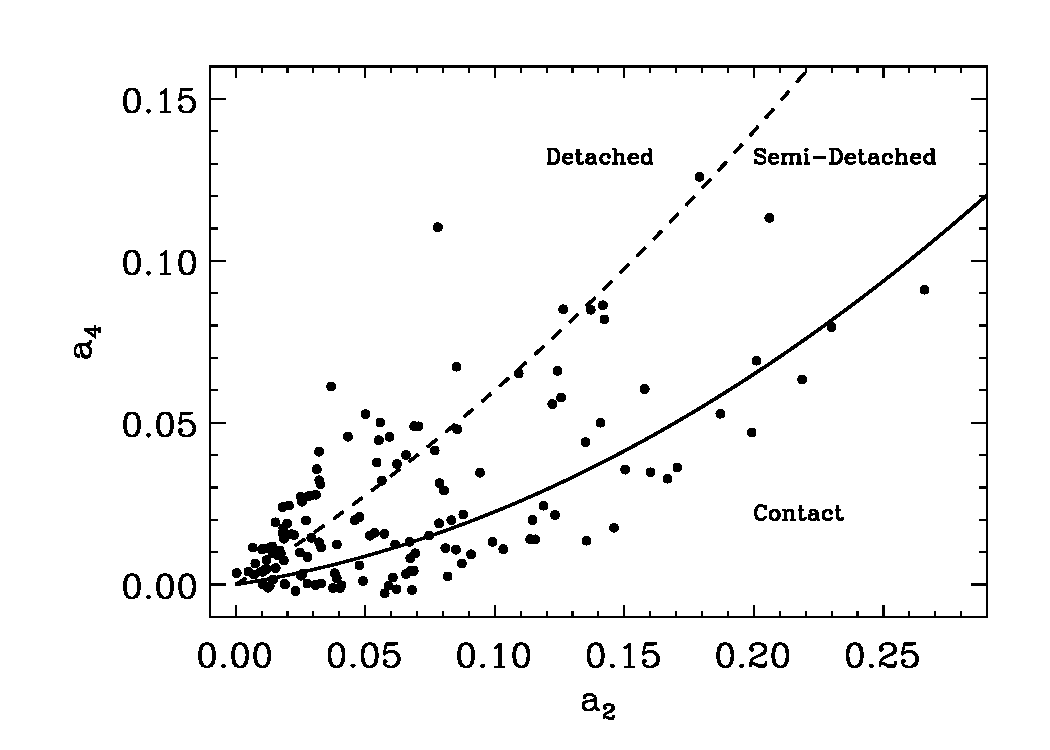
\includegraphics[width=3.5in]{new_plots/four_a2a4}
\caption{Fourier modes used to select between eclipsing binaries and pulsators (top) and different classes of eclipsing binaries (bottom).}
\label{four_bb}
\end{figure}


\begin{figure}[]
\centering
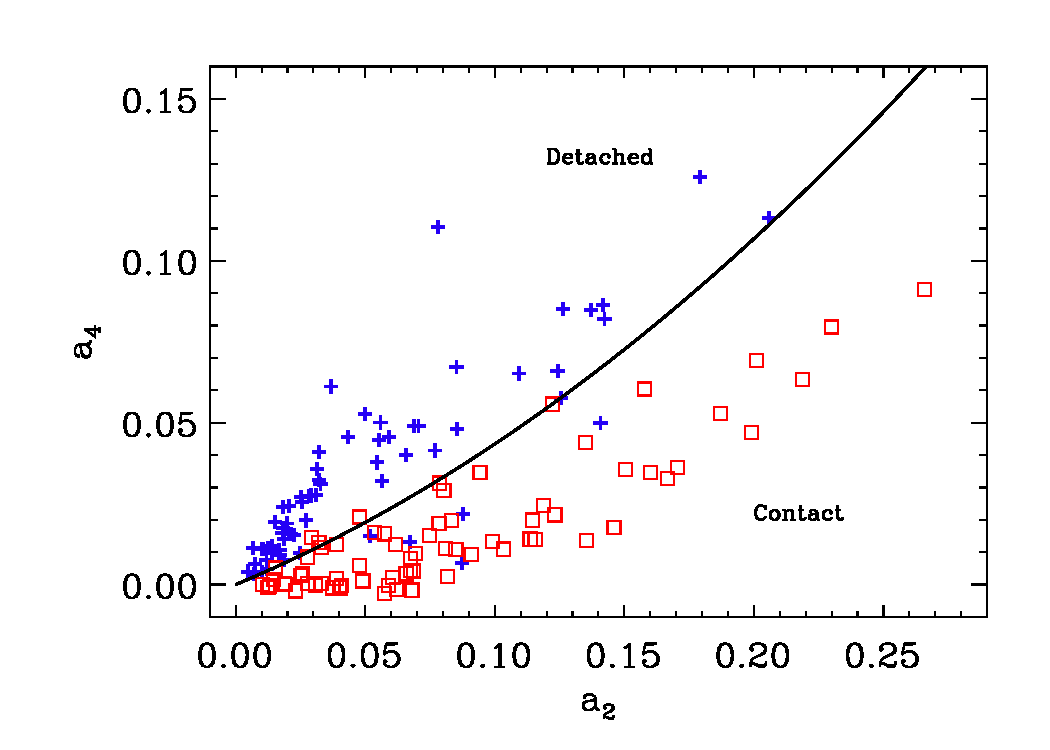
\includegraphics[width=3.5in]{new_plots/four_a2a4_jrad}
\caption{My classification of different classes of eclipsing binaries (bottom). separation given in text}
\label{four_bb2}
\end{figure}




%%%%%%%%%%%%%%%%%%%%%%%%%
\section{Binaries}
We found 100 binaries, need a histogram of their periods. We recover nearly all the binaries from Plavchan's early work (8/23 missed so far)

match to new paper by J Parks (2012)




Using our by-hand classification, we can define the best line of delineation between contact and detached eclipsing binaries in this Fourier space. \citet{rucinski1997b} used $a_4< a_2(0.3 + a_2)$ to separate these two populations using OGLE light curves. We had 64 detached, 72 detached by hand classified. We used a brute-force approach to solve for the coefficient $C$ in 
\begin{equation}
a_4 = a_2(C + a_2)\,,
\end{equation}
calculating the fraction of each population correctly classified at each iteration. We used values of $c$ ranging from 0 to 1, in steps of 0.001. The best degree of separation was found for $C=0.334$, yielding 95\% completeness for contact binaries, and 92\% completeness for detached systems.


the final sample of classified objects were: XX contact binaries, YY semi-detached, ZZ detached, 12 pulsators, and 25 quasi-periodic oddballs. a selection of the LPV/QPVs are given in Figure \ref{ll} (MOVE UP). this matched with total rates of these objects from other surveys? Check out OGLE or ASAS, have they got similar proportions of binaries and rr Lyr?




for every binary, estimate the spectral type based on Davenport (2013 in prep) color-locus. use SDSS colors for stars w/ matches, and WISE colors for everything else (hopefully). this provides a much improved ability to select dM's, rather than a broad-brush color box previously used. We find XX eclipsing binaries with M dwarf colors (g-i between 2 and 3, or whatever). are any of these detached binaries? if so, gold mine. 5 of these are new, we have missed 5 from Plavchan work. Since very in depth effort been put towards rho Oph field, haven't focused on these fields.

55 contact, 43 semi-detached, 48 detached binaries based on the equations

\begin{figure}[]
\centering
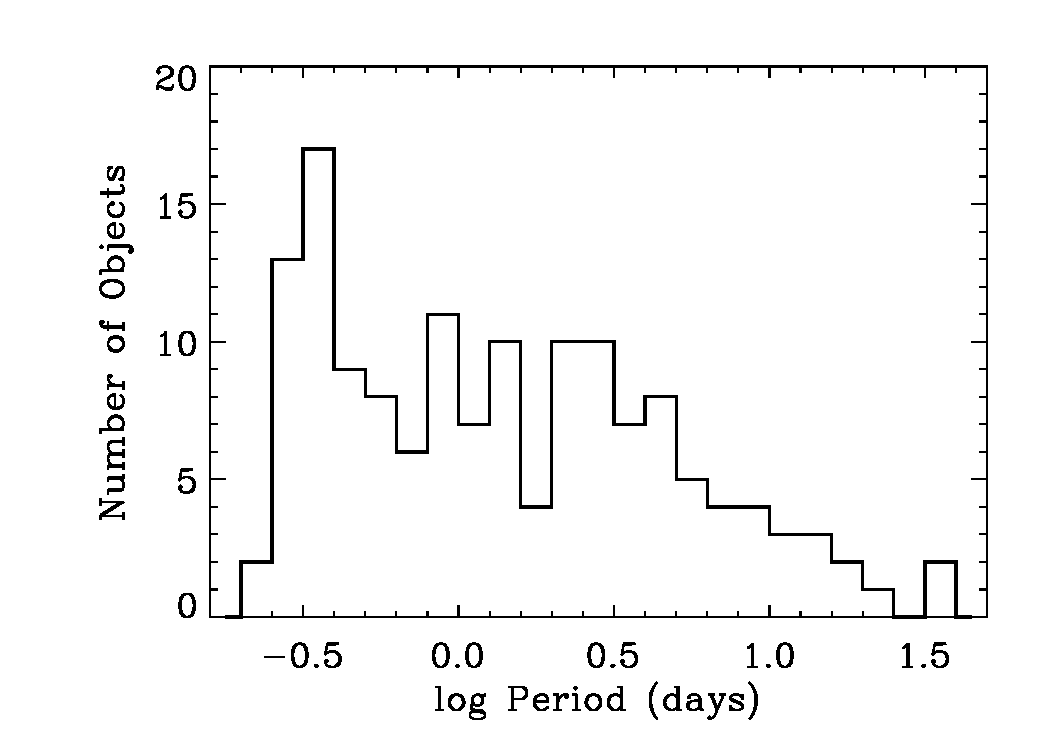
\includegraphics[width=3.5in]{new_plots/bb_perhist}
\caption{Distribution of periods for objects selected as binaries. Note the sharp cutoff at $log P \sim -0.6$, $P \sim 0.25$ days.}
\label{perhist}
\end{figure}



\begin{figure}[!h]
\centering
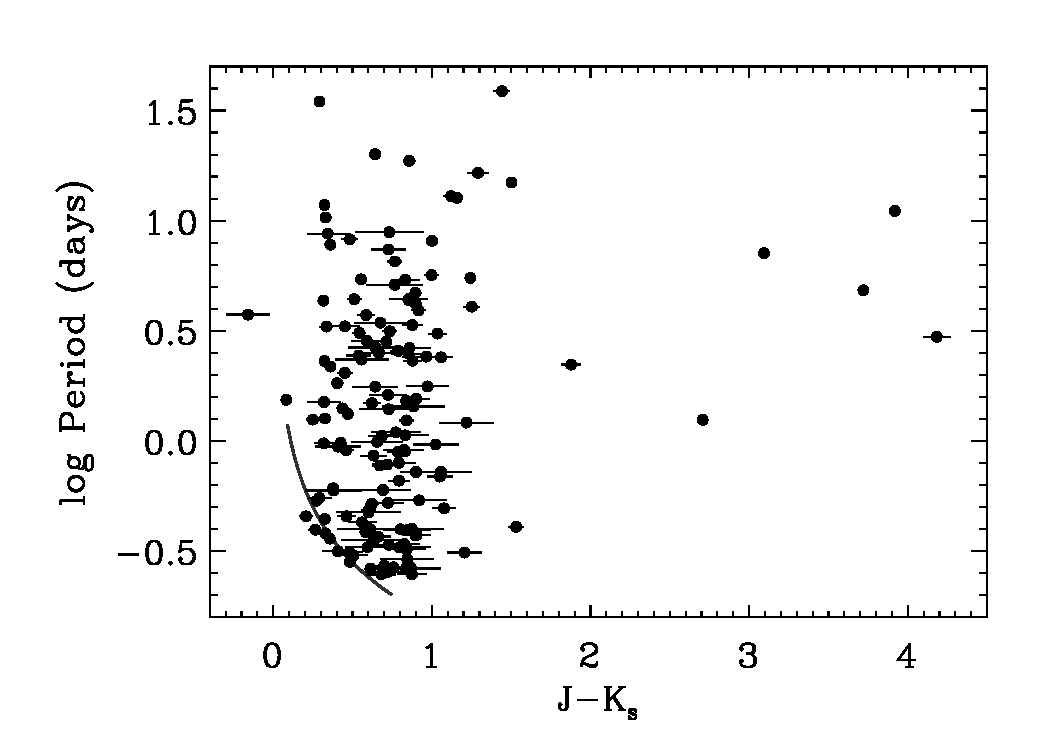
\includegraphics[width=3.5in]{new_plots/color_period_bb}
\caption{Period versus median colors for objects selected as binaries. The photometry was not corrected for reddening. The power law short period contact binary limit from \cite{deb2011} is shown for comparison (solid gray line). NEW COLOR FOR LINE, MAKE SYMBOLS DIFFERENT USING CLASSIFICATION FROM FIGURE 2}
\label{periods}
\end{figure}


examples of each type

\begin{figure*}[]
\centering
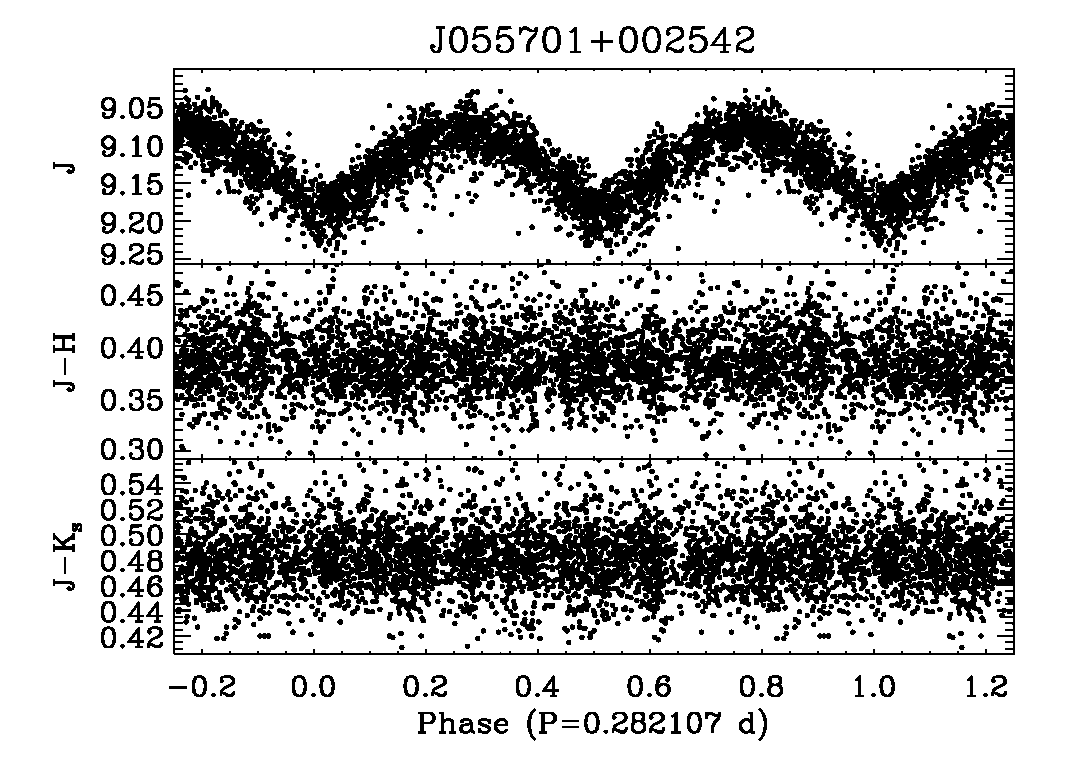
\includegraphics[width=2.0in]{new_plots/bb1_6}
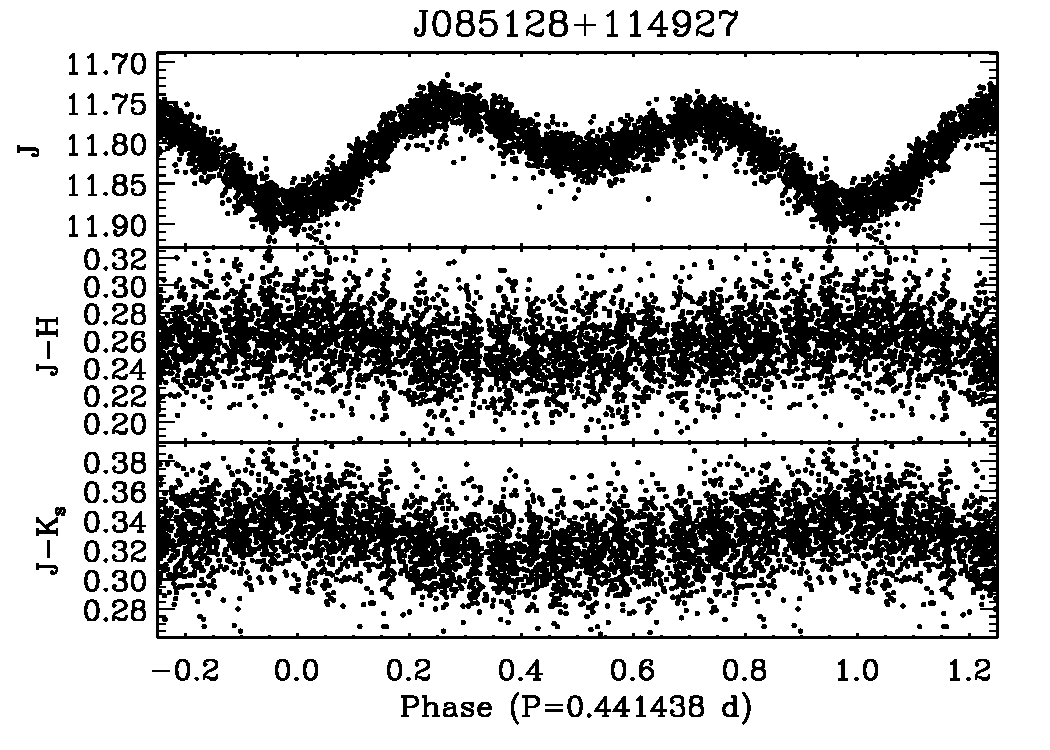
\includegraphics[width=2.0in]{new_plots/bb1_7}
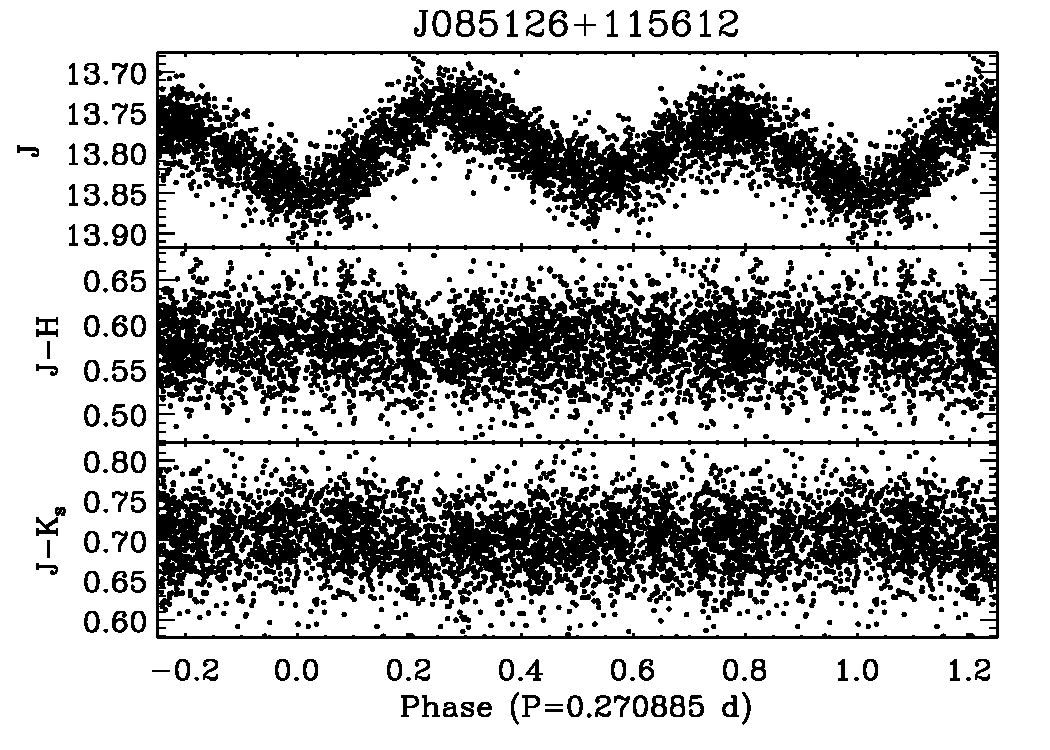
\includegraphics[width=2.0in]{new_plots/bb1_8}
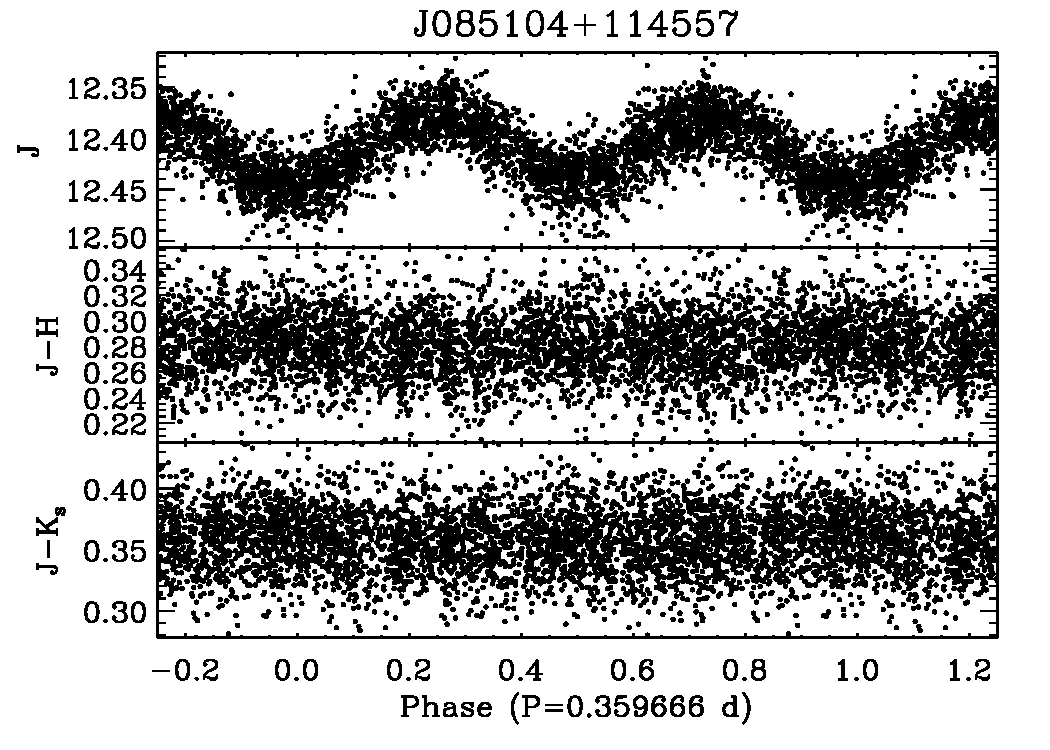
\includegraphics[width=2.0in]{new_plots/bb1_10}
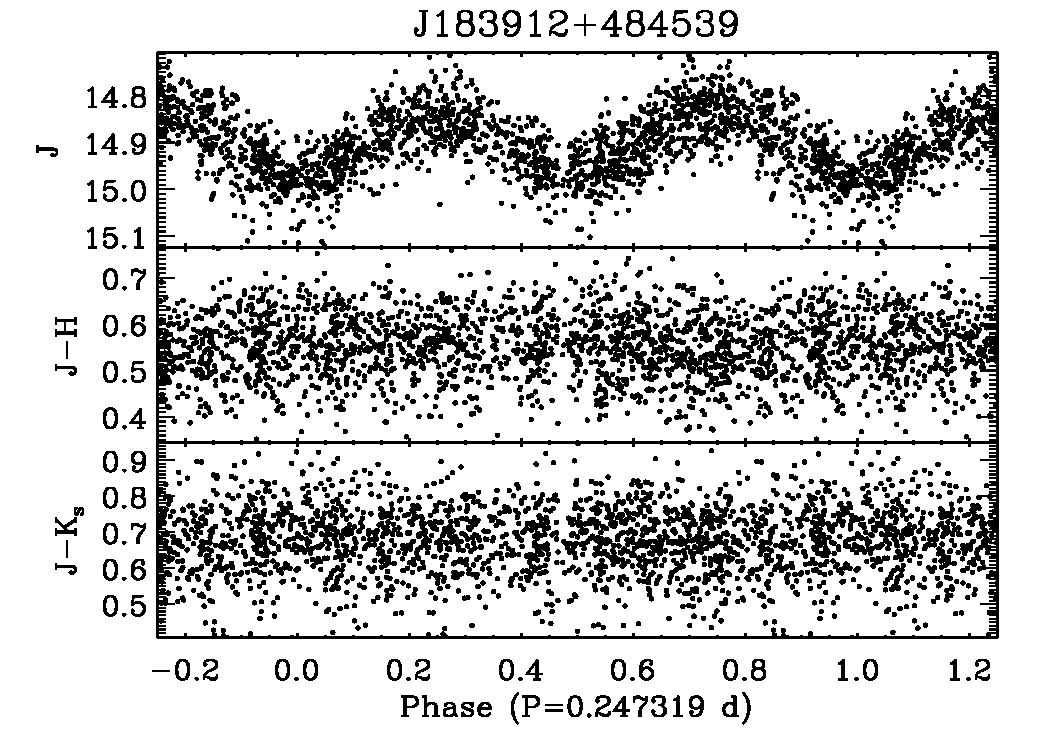
\includegraphics[width=2.0in]{new_plots/bb1_13}
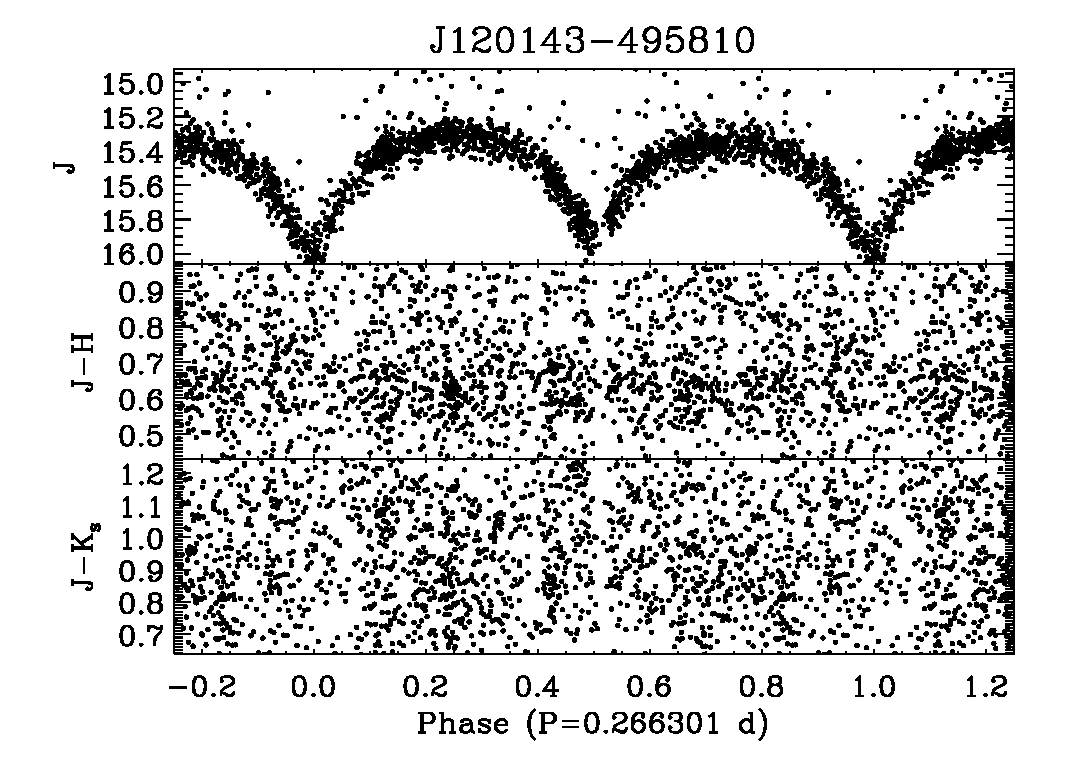
\includegraphics[width=2.0in]{new_plots/bb1_15}
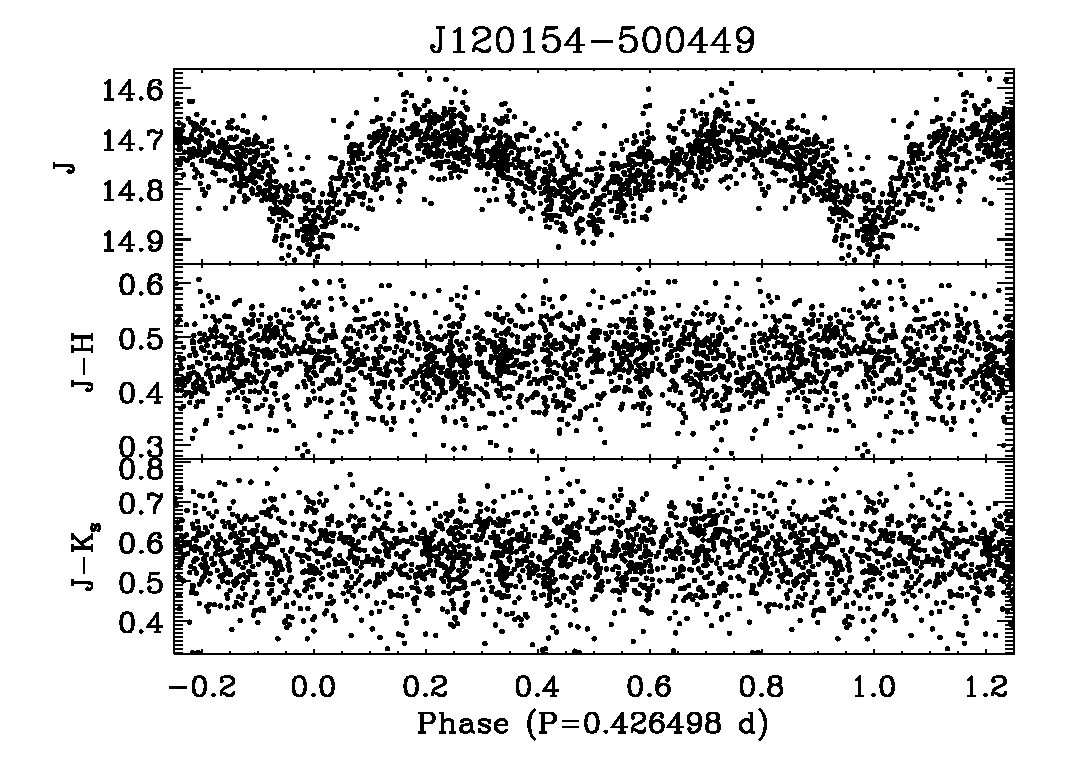
\includegraphics[width=2.0in]{new_plots/bb1_16}
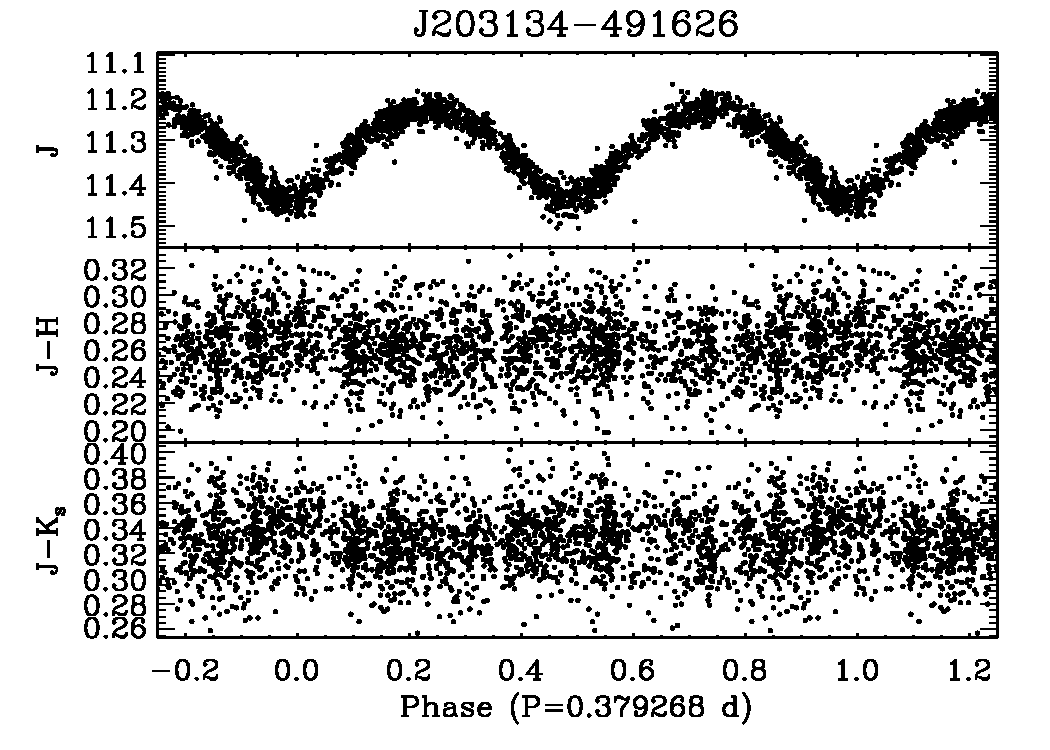
\includegraphics[width=2.0in]{new_plots/bb1_17}
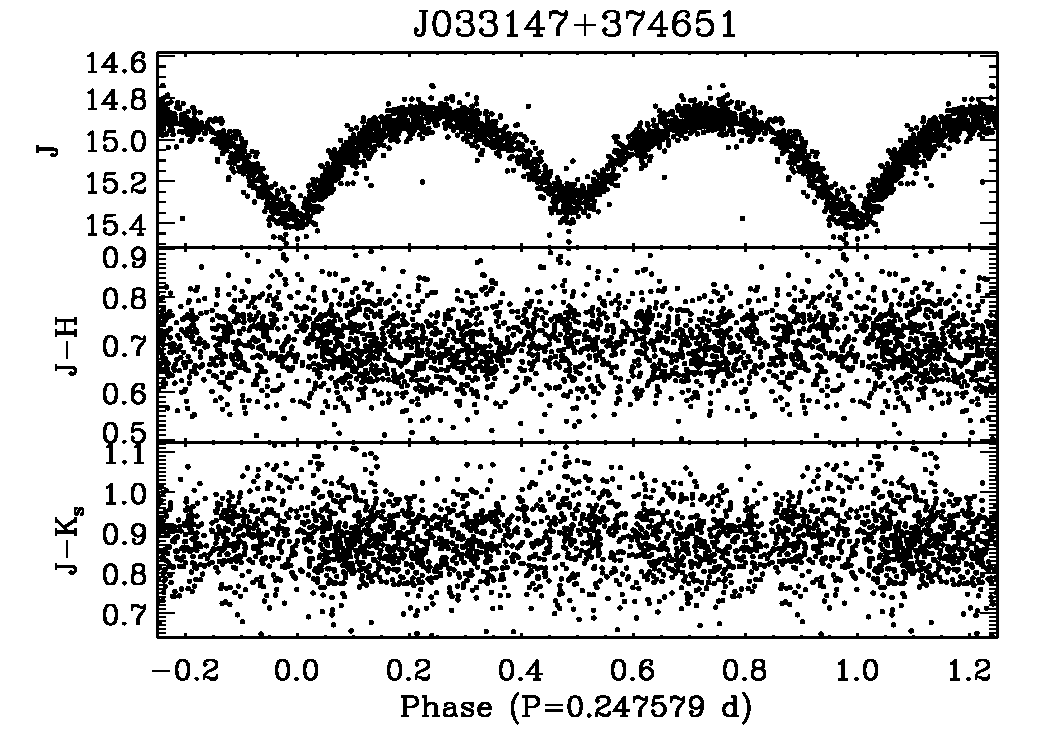
\includegraphics[width=2.0in]{new_plots/bb1_18}
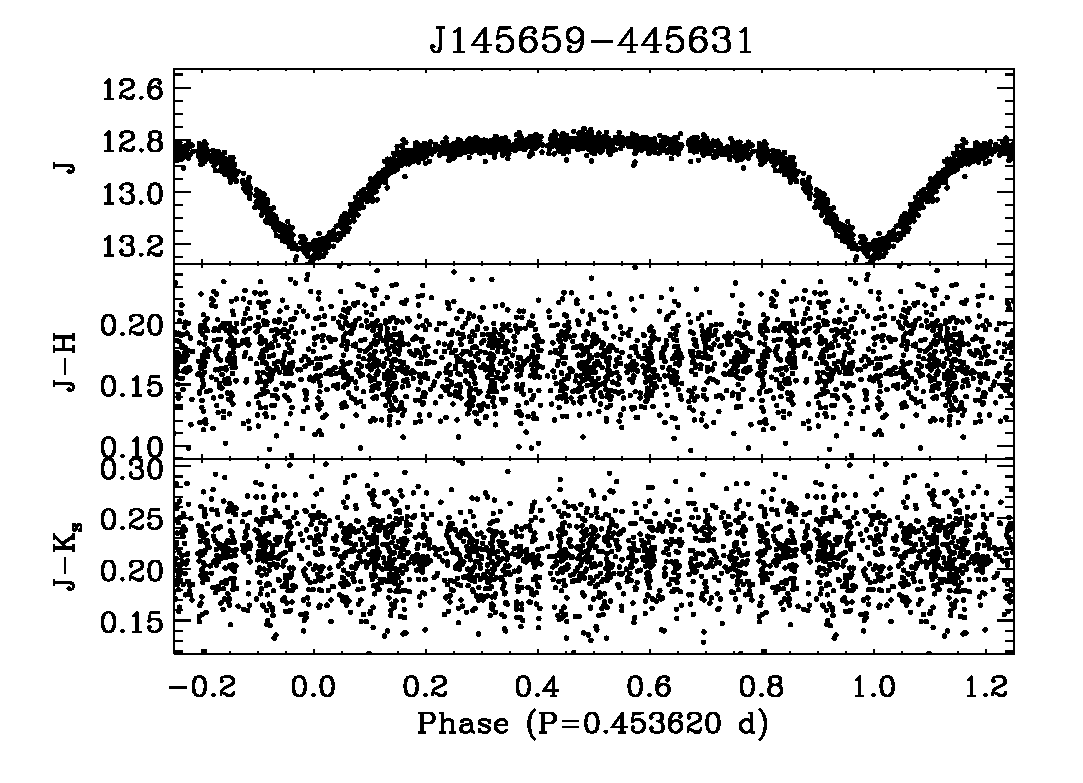
\includegraphics[width=2.0in]{new_plots/bb1_21}
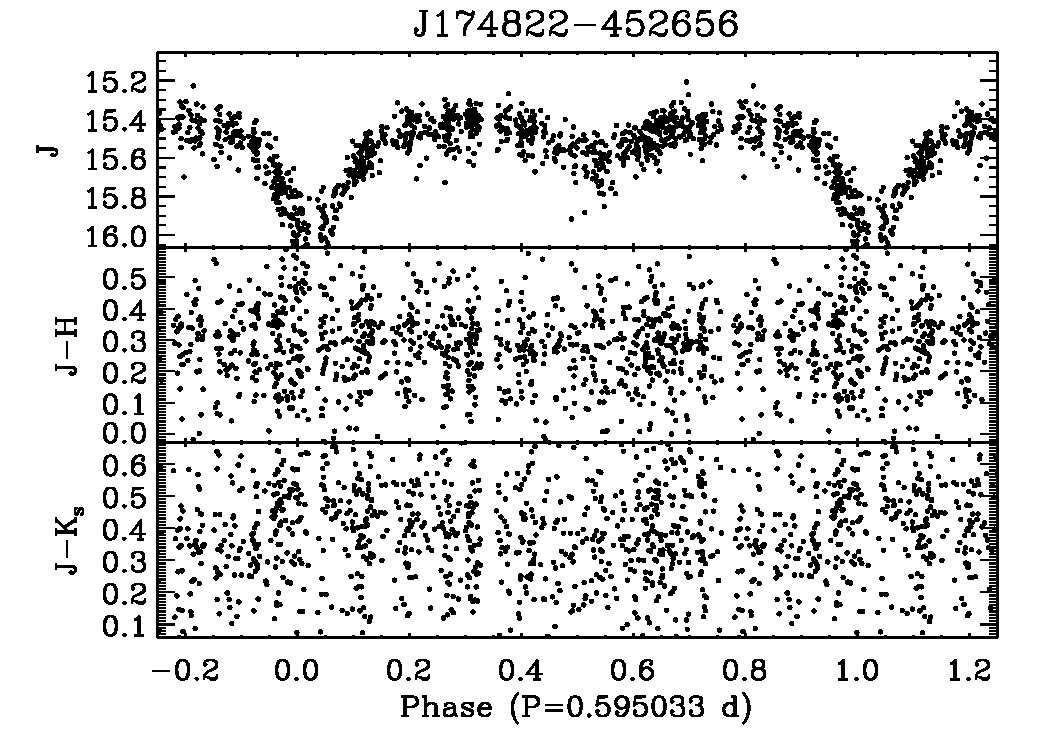
\includegraphics[width=2.0in]{new_plots/bb1_28}
\caption{contact binaries}
\label{bin1}
\end{figure*}


\begin{figure*}[]
\centering
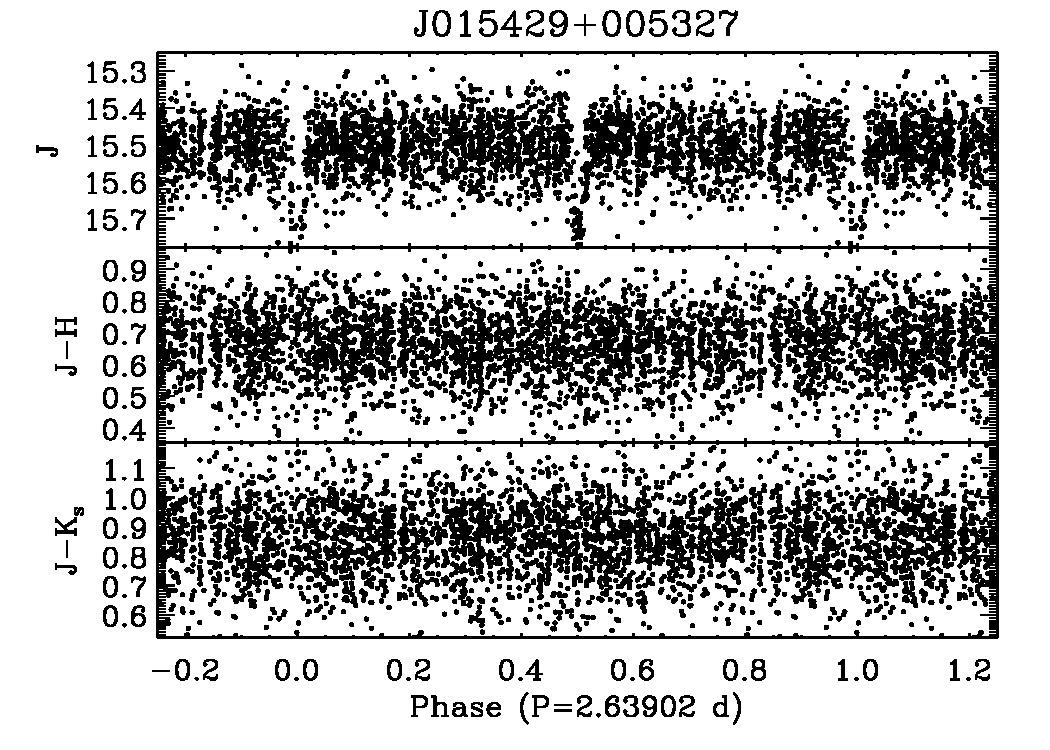
\includegraphics[width=2.0in]{new_plots/bb3_0}
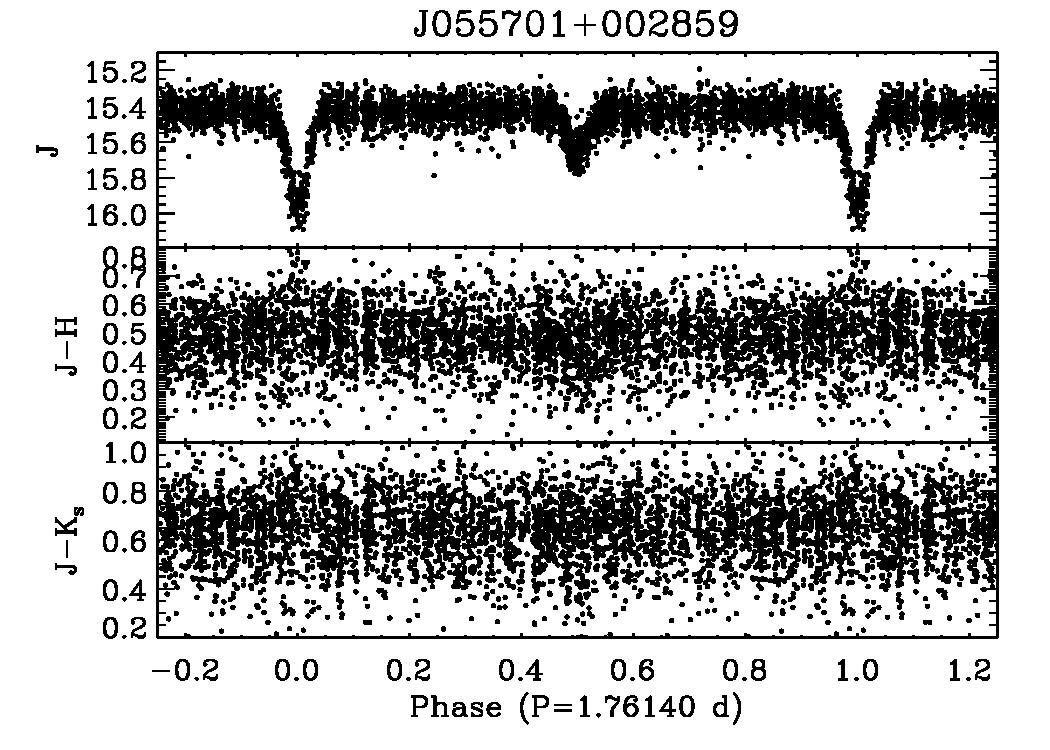
\includegraphics[width=2.0in]{new_plots/bb3_2}
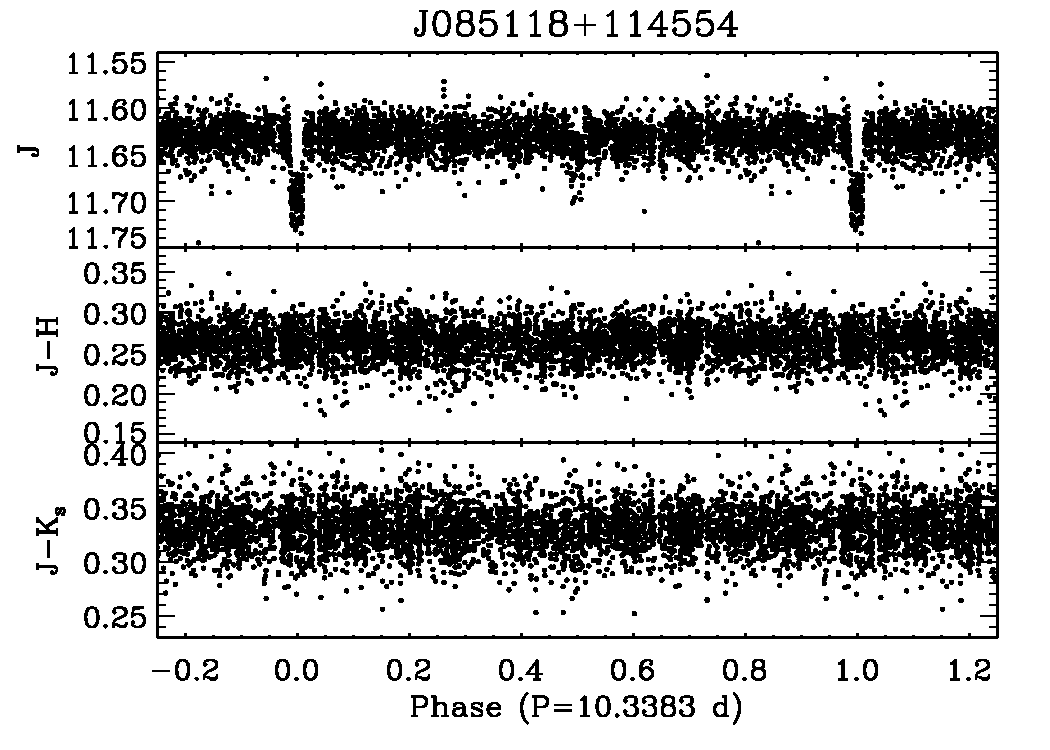
\includegraphics[width=2.0in]{new_plots/bb3_3}
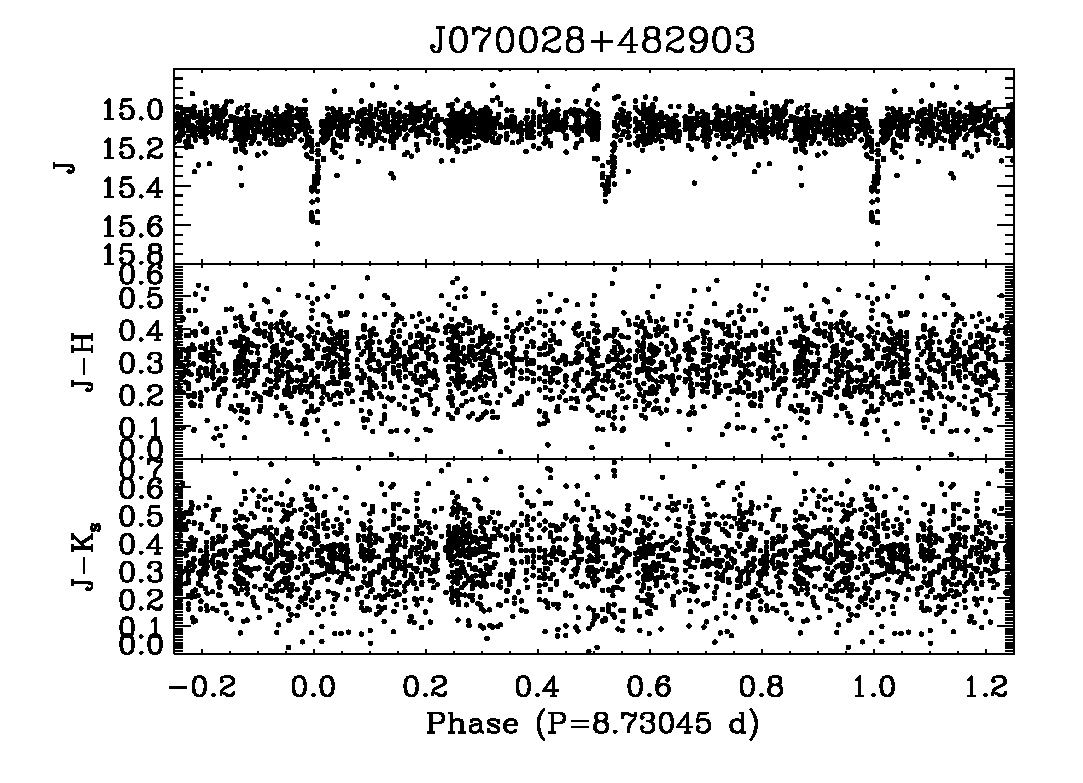
\includegraphics[width=2.0in]{new_plots/bb3_6}
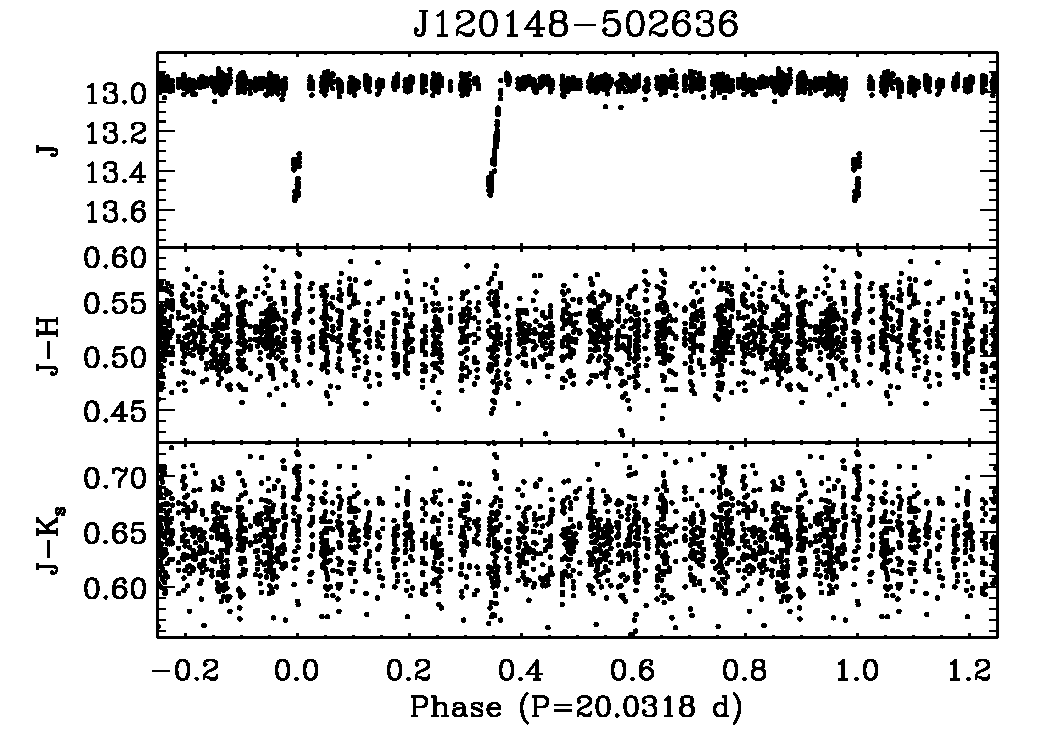
\includegraphics[width=2.0in]{new_plots/bb3_10}
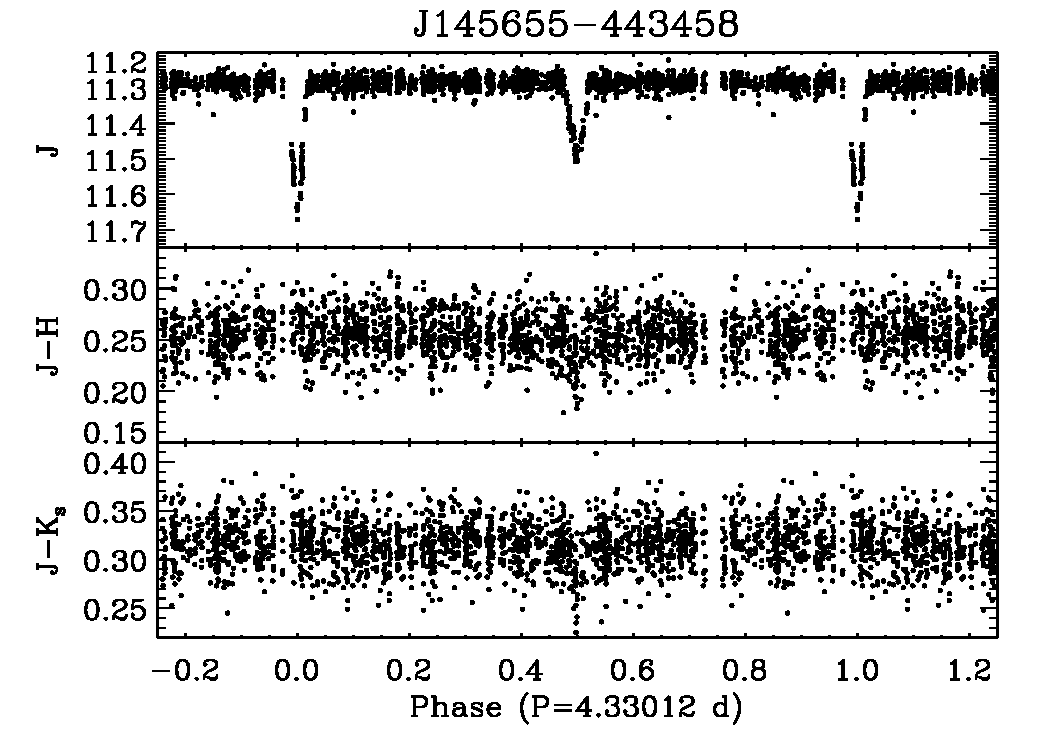
\includegraphics[width=2.0in]{new_plots/bb3_14}
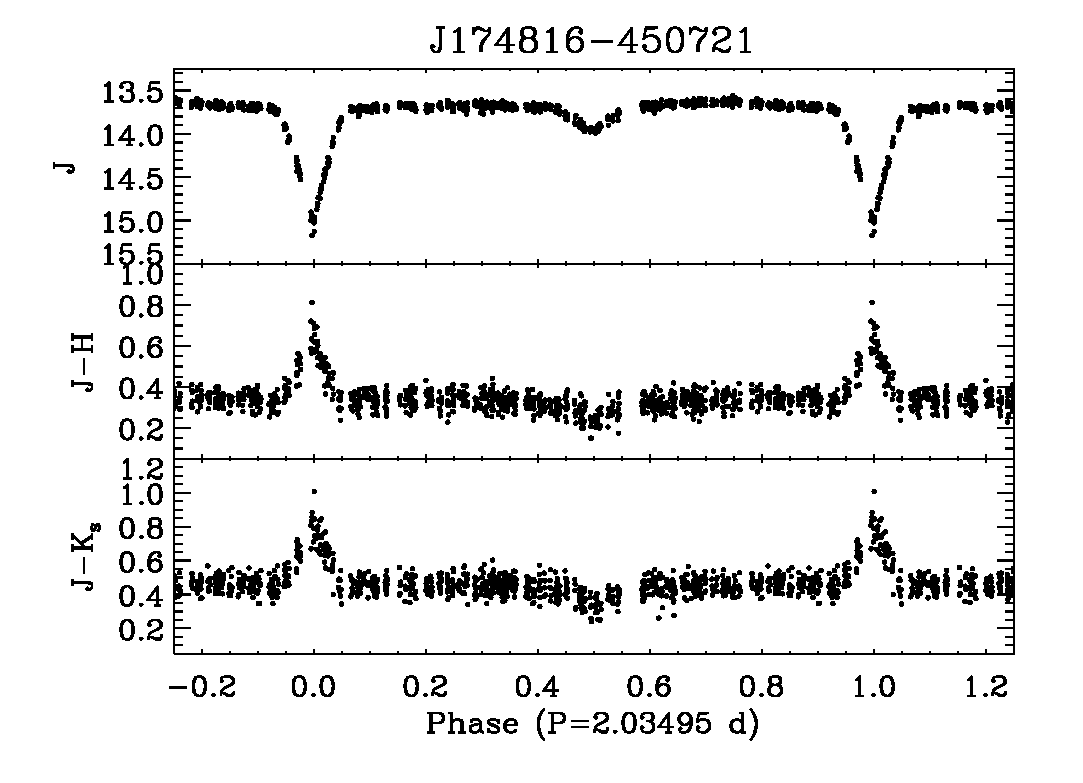
\includegraphics[width=2.0in]{new_plots/bb3_16}
\caption{detached binaries}
\label{bin1}
\end{figure*}


%the shortest period (semi-) detached binary
%\begin{figure}[]
%\centering
%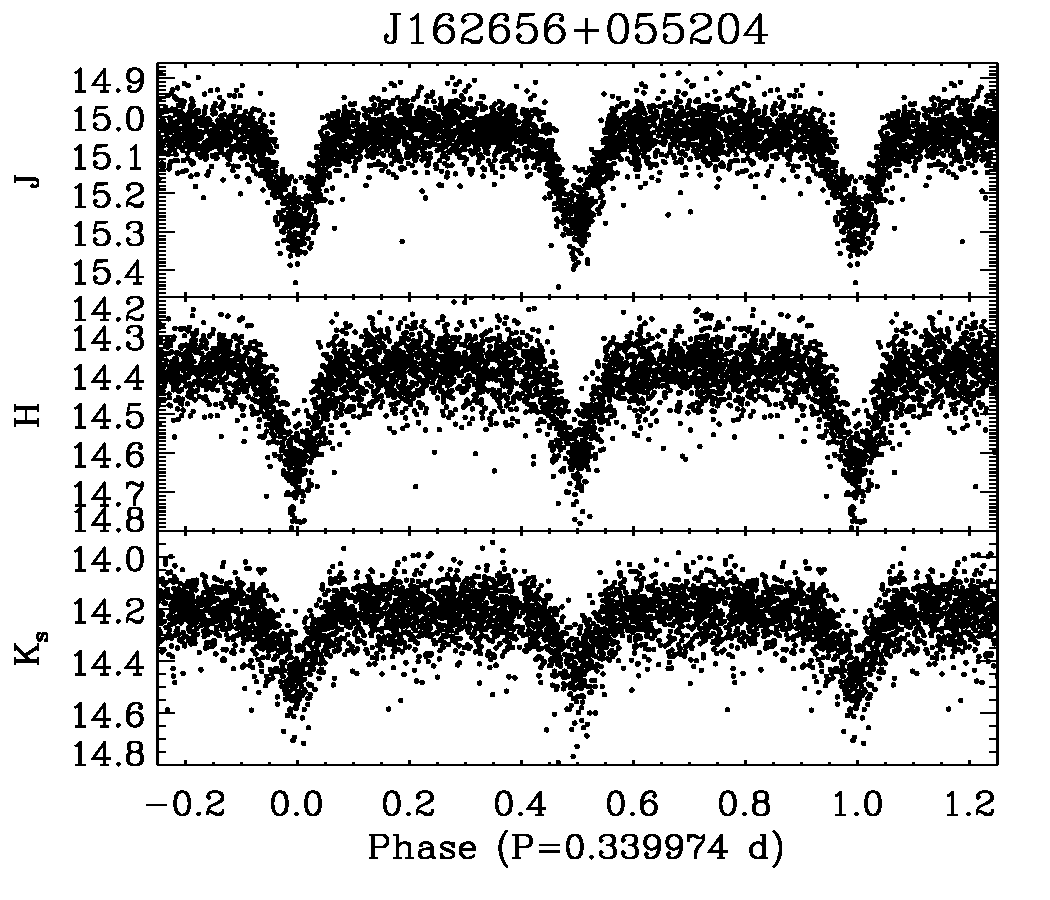
\includegraphics[width=3.0in]{plots/shortest_sep}
%\caption{detached binaries}
%\label{shortbin}
%\end{figure}




%%%%%%%%%%%%%%%%%%%%%%%%%
\section{Pulsators}
Infrared observations of radial pulsating stars was first performed by \cite{wisniewski1968}, and detailed characterization was done for Cepheid variables by \cite{mcgonegal1982} and for RR Lyr variables by \cite{longmore1985}

$K$-band templates first derived in \citet{jones1996}

RR Lyr type variables belong broadly to two classes: RRab and RRc, defined by their light curve morphologies \citep{bailey1902}

\citet{sollima2008} produced $JHK_s$ light curves for the prototypical star, RR Lyr.

limited numbers found in the NIR, usually many few numbers of epochs and phase coverage \citep[e.g.][]{delprincipe2005}


-- outline of section --
these NIR light curves provide benchmarks for several classes of radial pulsating periodic variables. phase coverage is excellent for most of these objects

we have the best Cepheid NIR light curve, best regular RR Lyr, a good $\delta$ Scu, and probably some RR a and RR b types (need to look up difference). this list was matched up against SIMBAD, only XX were previously known about.

No Blazko variables - though should check the known sample to see if any have it and don't show it here.

the list is given in Table X, including distances computed using de-reddened and period-mag relations (CITE)

\subsection{Effects of Shocks}
the light curves can also be folded in to the color-mag space, and medians show kinks. we do this for all the objects.



\begin{figure}[]
\centering
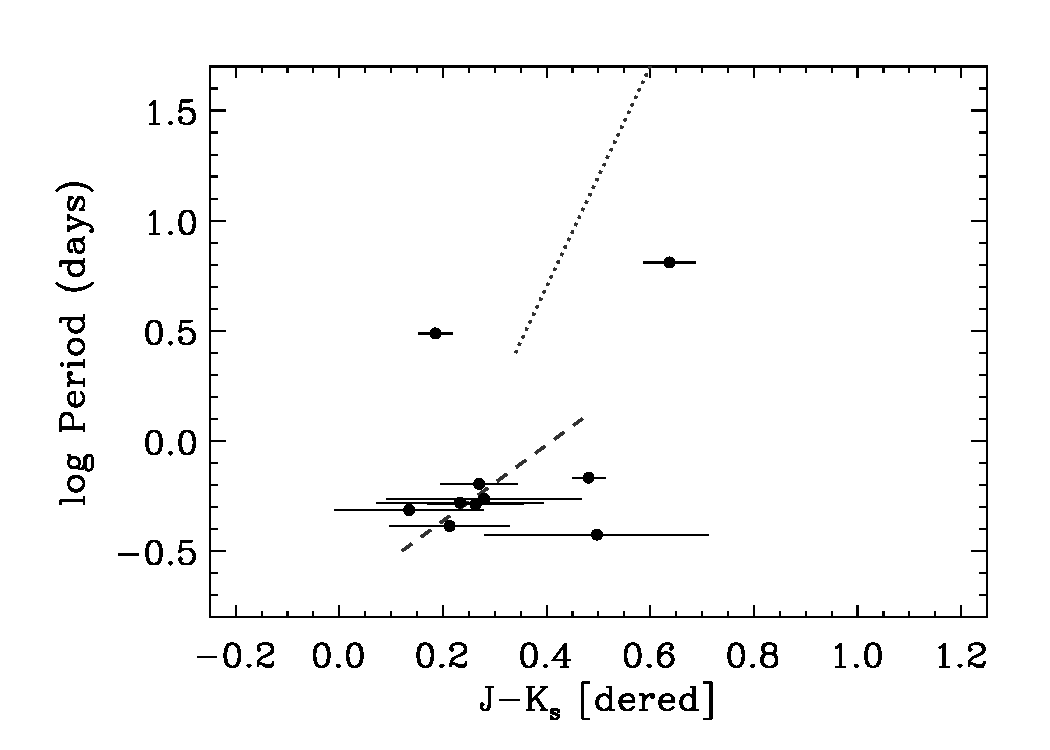
\includegraphics[width=3.0in]{new_plots/color_period_rr}
\caption{17 radial pulsator variables. dashed line is theoretical prediction from \citet{catelan2004} with Z=0.001 (no discernible dependence on Z) dotted line is for Cepheids, from ...}
\label{rr_color_period}
\end{figure}


\begin{figure}[]
\centering
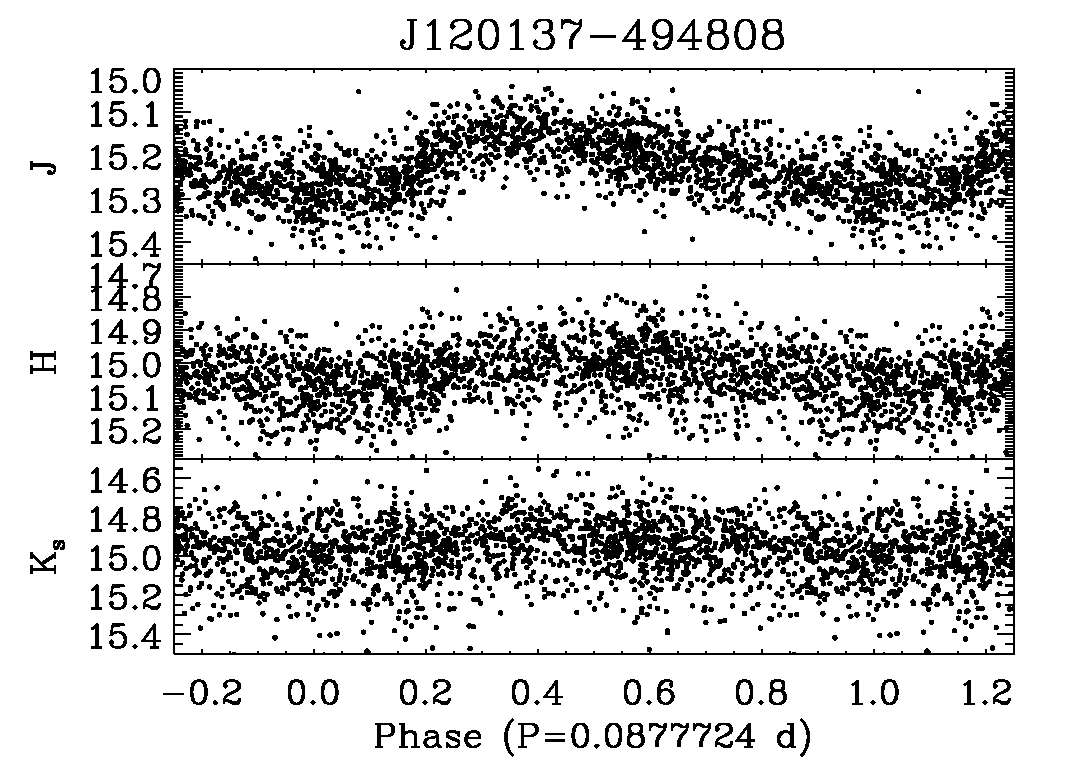
\includegraphics[width=3.0in]{new_plots/rr_0}
\caption{$\delta$ Scu variable}
\label{rrshort}
\end{figure}


\begin{figure}[]
\centering
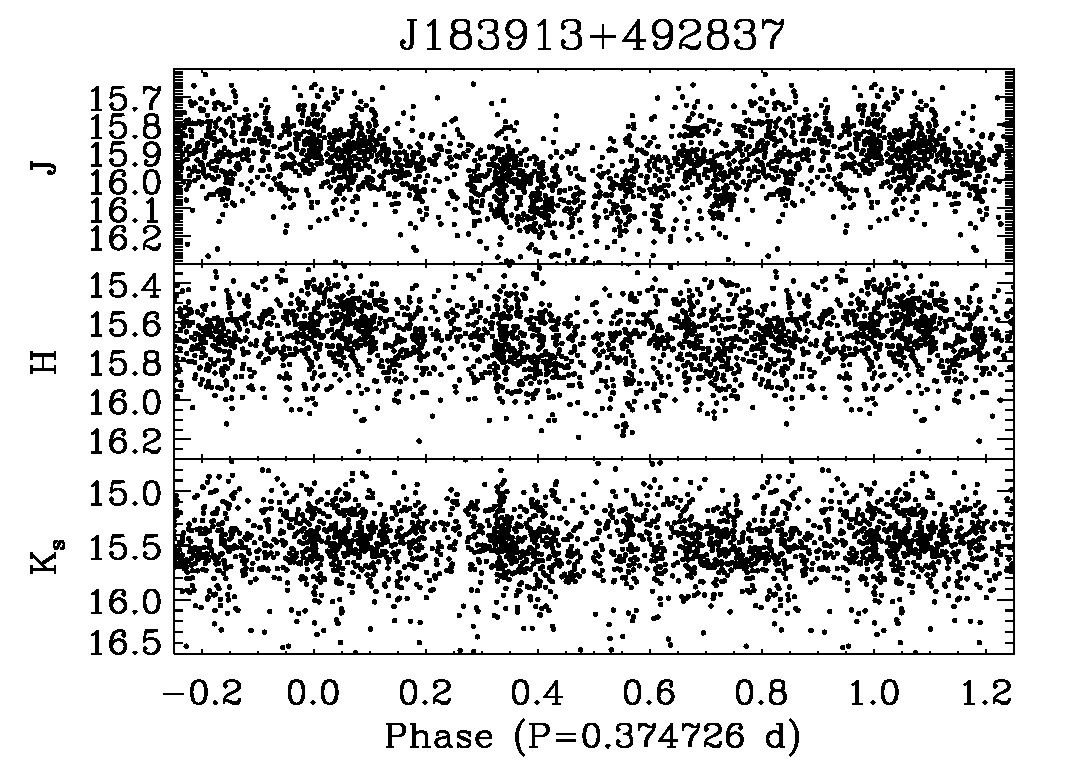
\includegraphics[width=3.0in]{new_plots/rr_1}
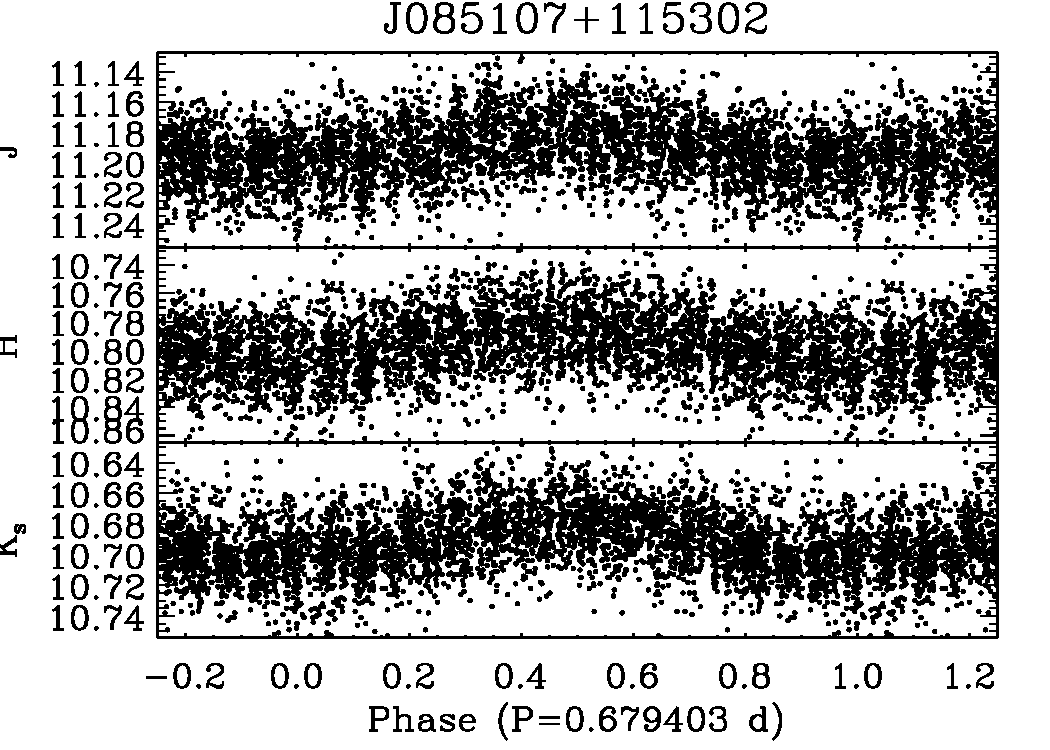
\includegraphics[width=3.0in]{new_plots/rr_8}
\caption{Pulsators with RRc-type light curves.}
\label{rrc}
\end{figure}

\begin{figure*}[]
\centering
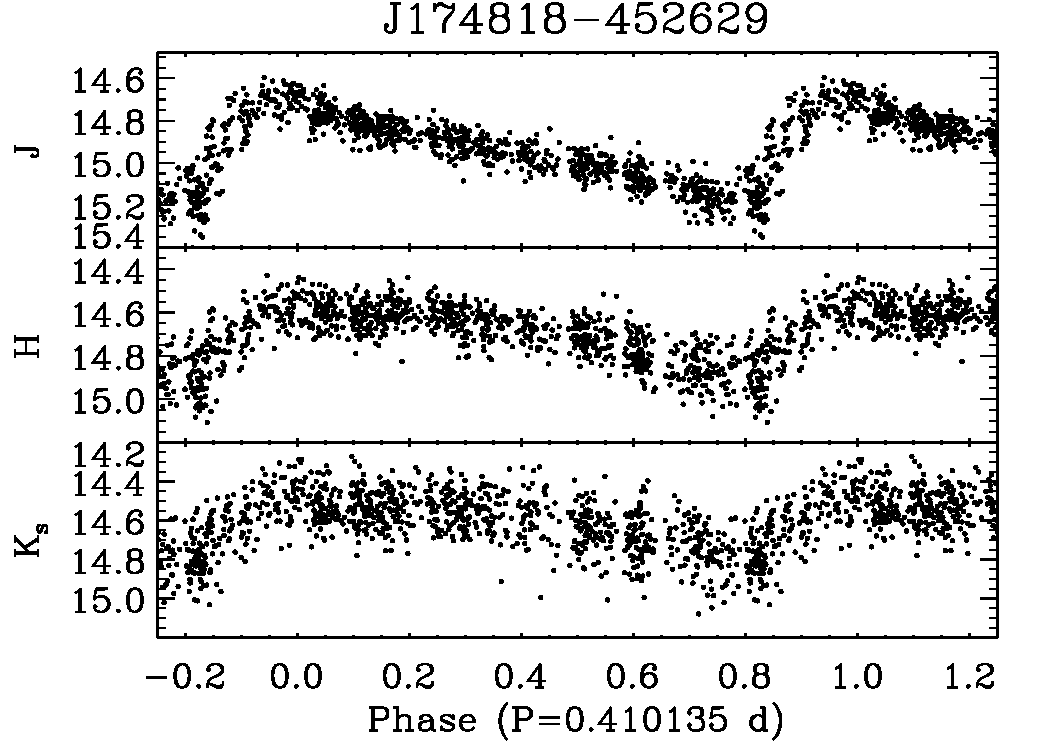
\includegraphics[width=2.0in]{new_plots/rr_2}
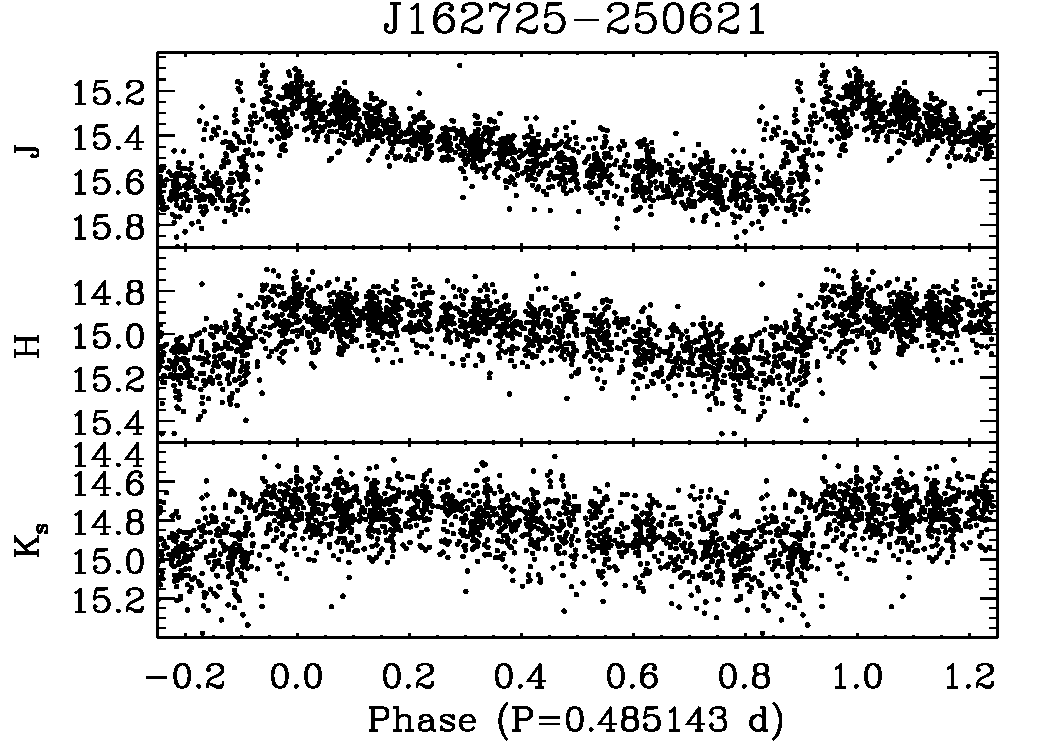
\includegraphics[width=2.0in]{new_plots/rr_3}
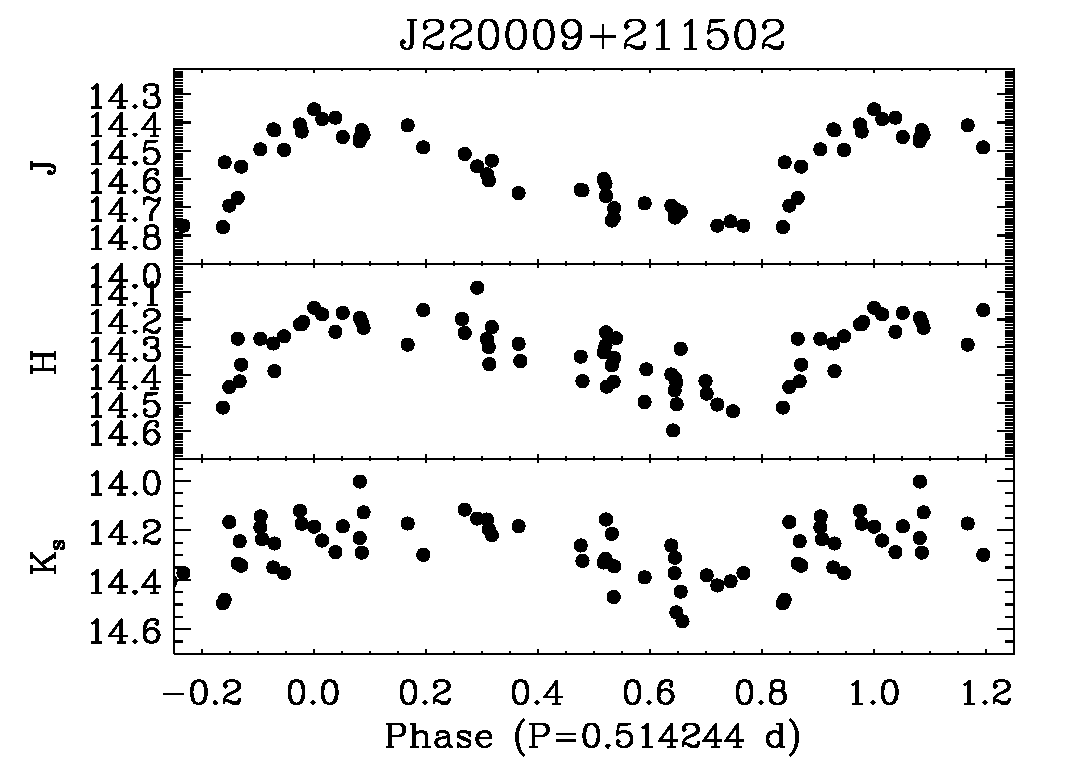
\includegraphics[width=2.0in]{new_plots/rr_4}\\
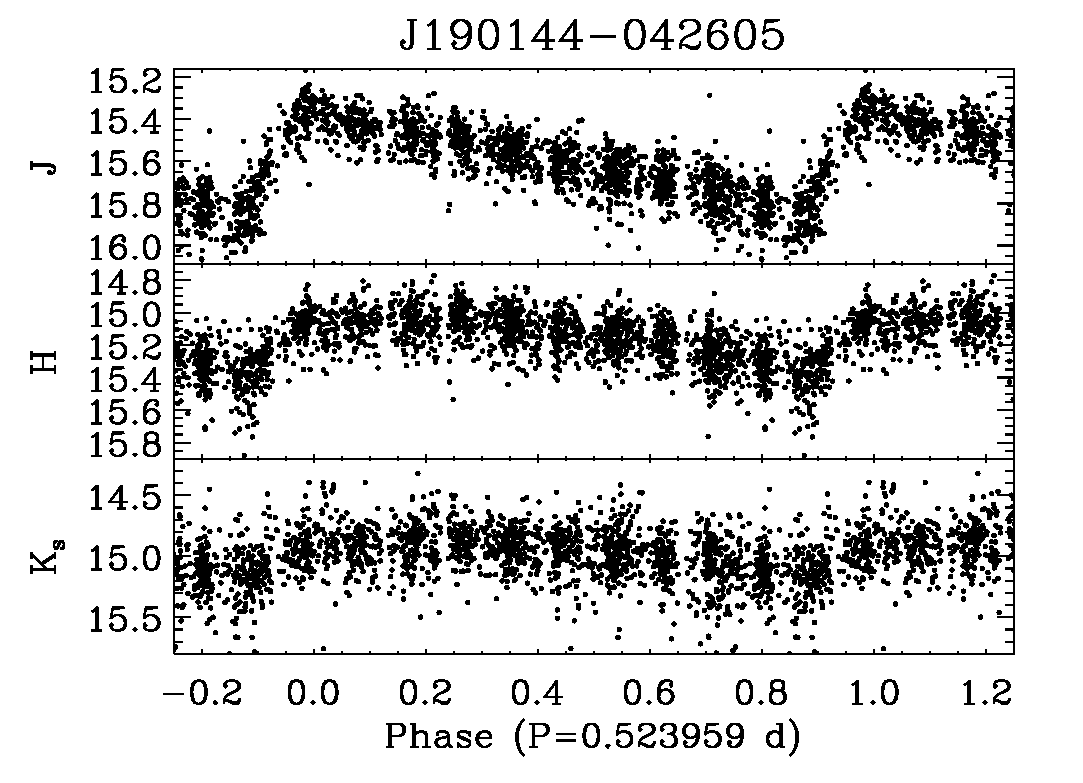
\includegraphics[width=2.0in]{new_plots/rr_5}
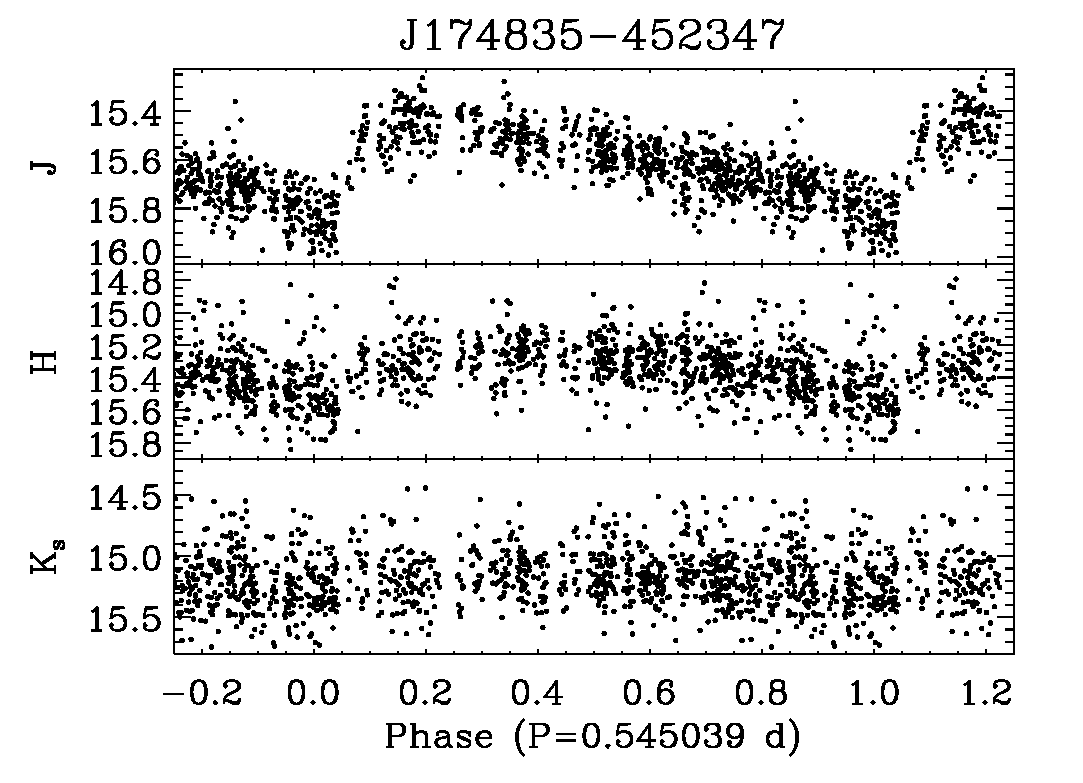
\includegraphics[width=2.0in]{new_plots/rr_6}
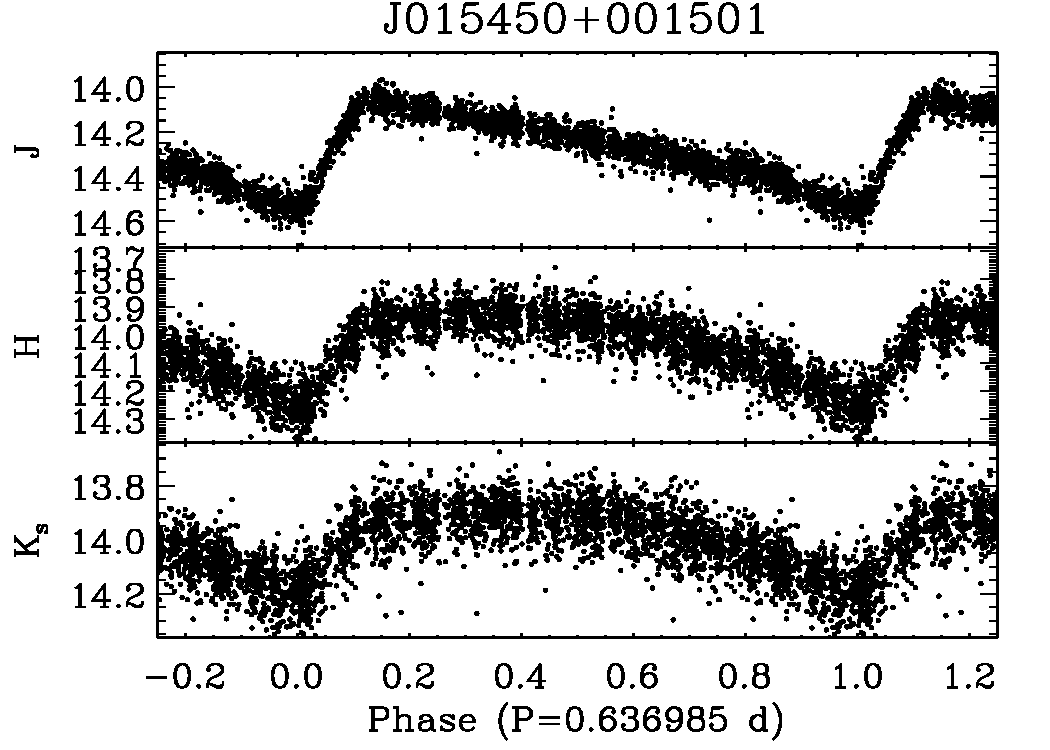
\includegraphics[width=2.0in]{new_plots/rr_7}
\caption{RRab-type variables}
\label{rrshort}
\end{figure*}

\begin{figure*}[]
\centering
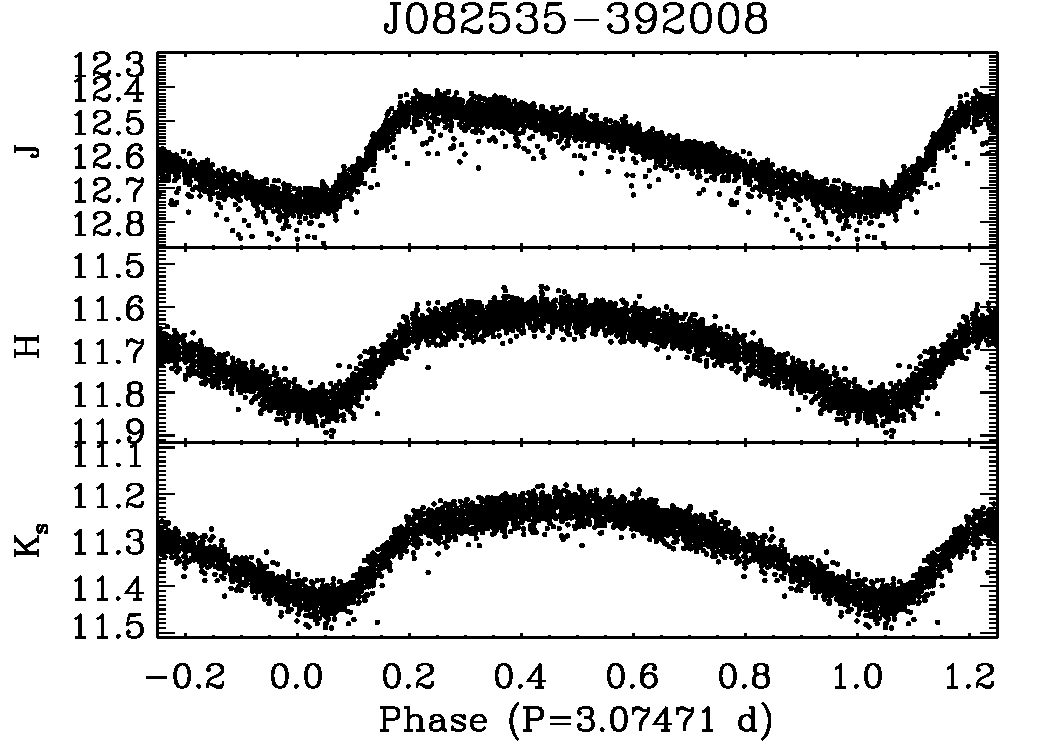
\includegraphics[width=2.5in]{new_plots/rr_9}
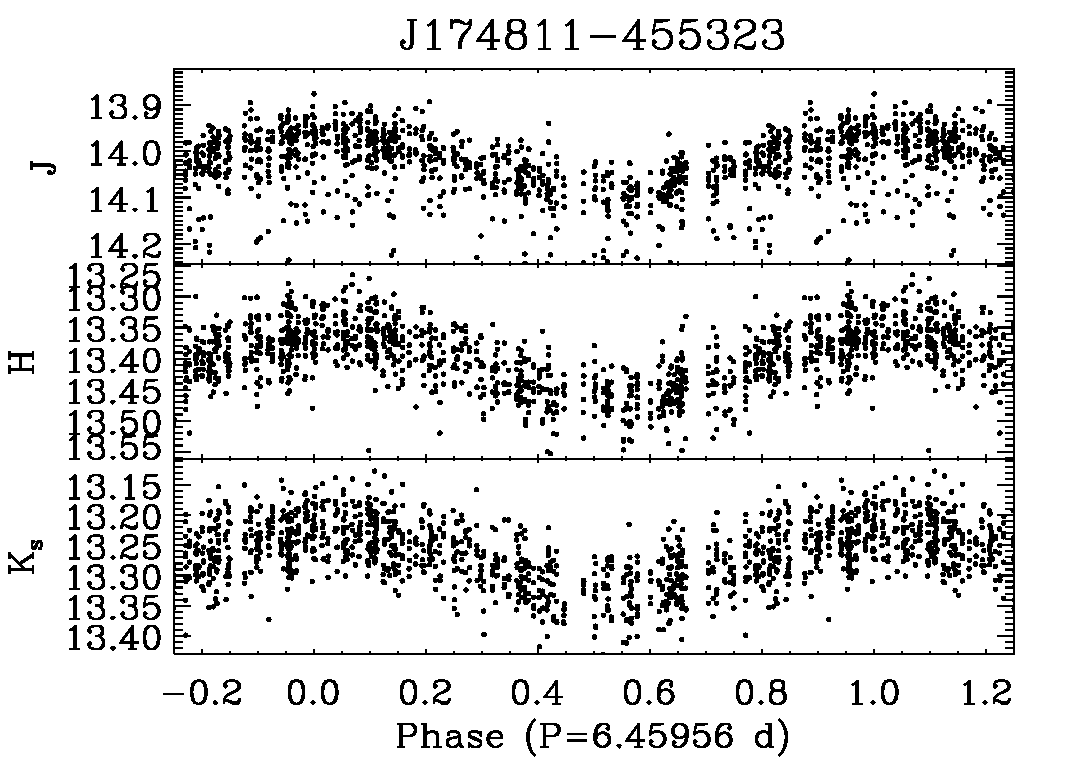
\includegraphics[width=2.5in]{new_plots/rr_10}
\caption{Pulsators (Cepheids)  with periods longer than 2 days}
\label{rrlong}
\end{figure*}


 

%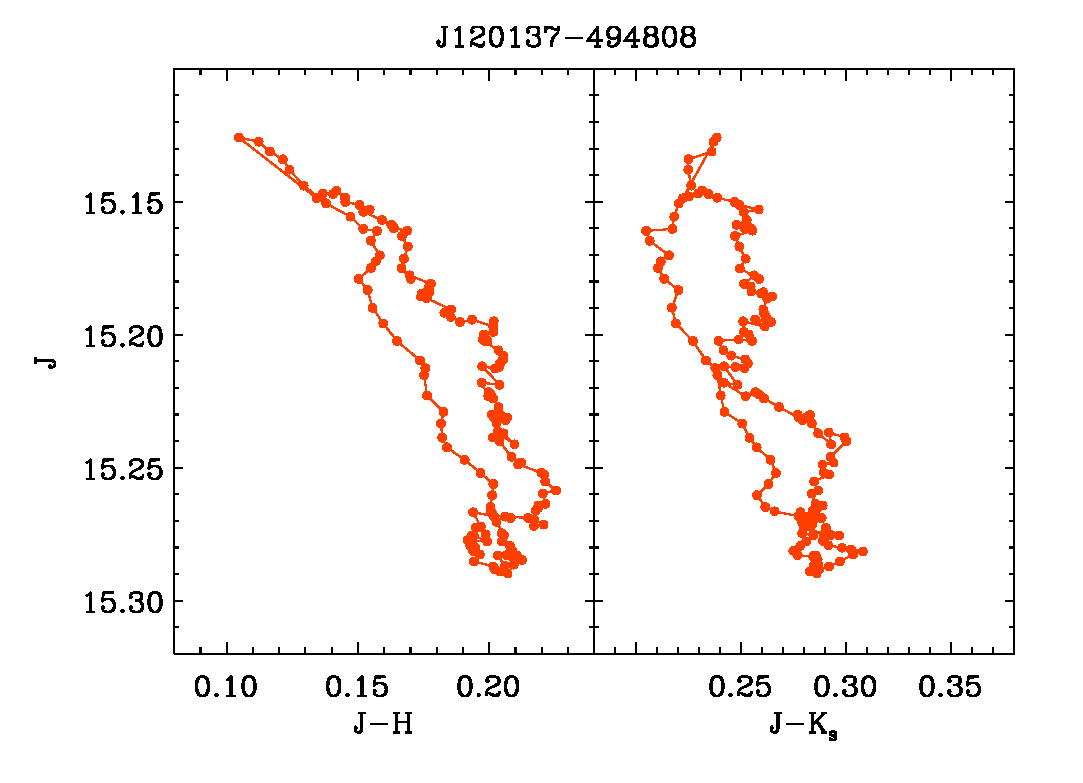
\includegraphics[width=2.0in]{new_plots/rr_cmd_0}
%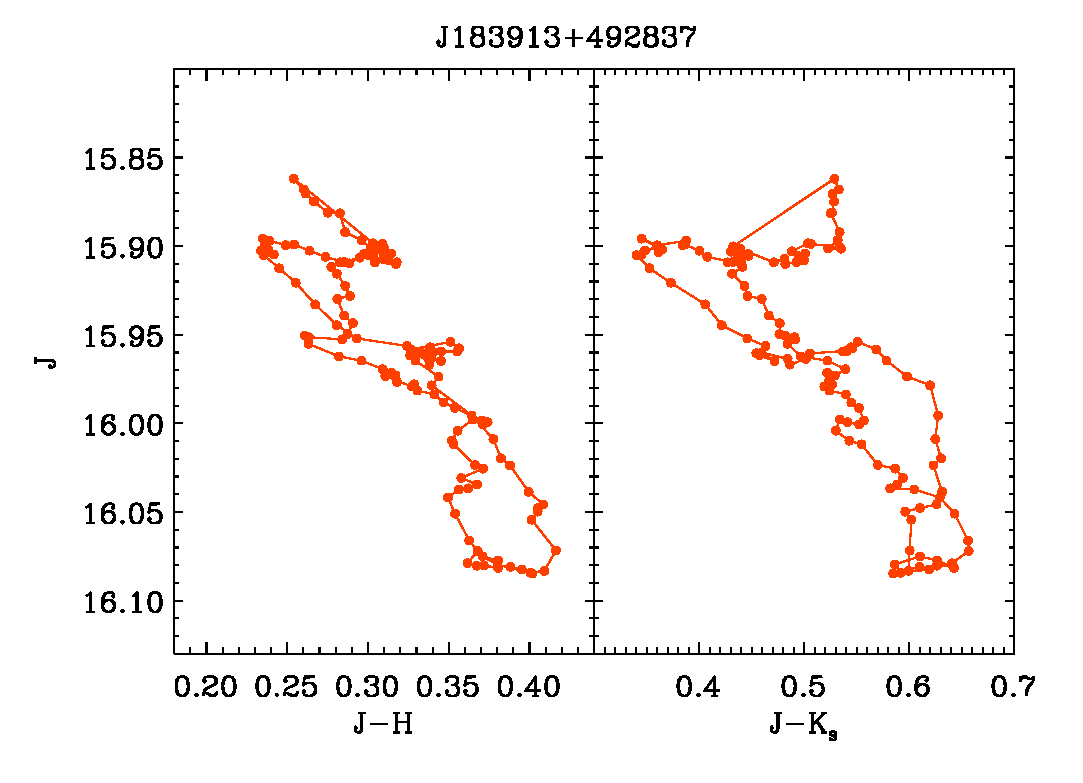
\includegraphics[width=2.0in]{new_plots/rr_cmd_1}
%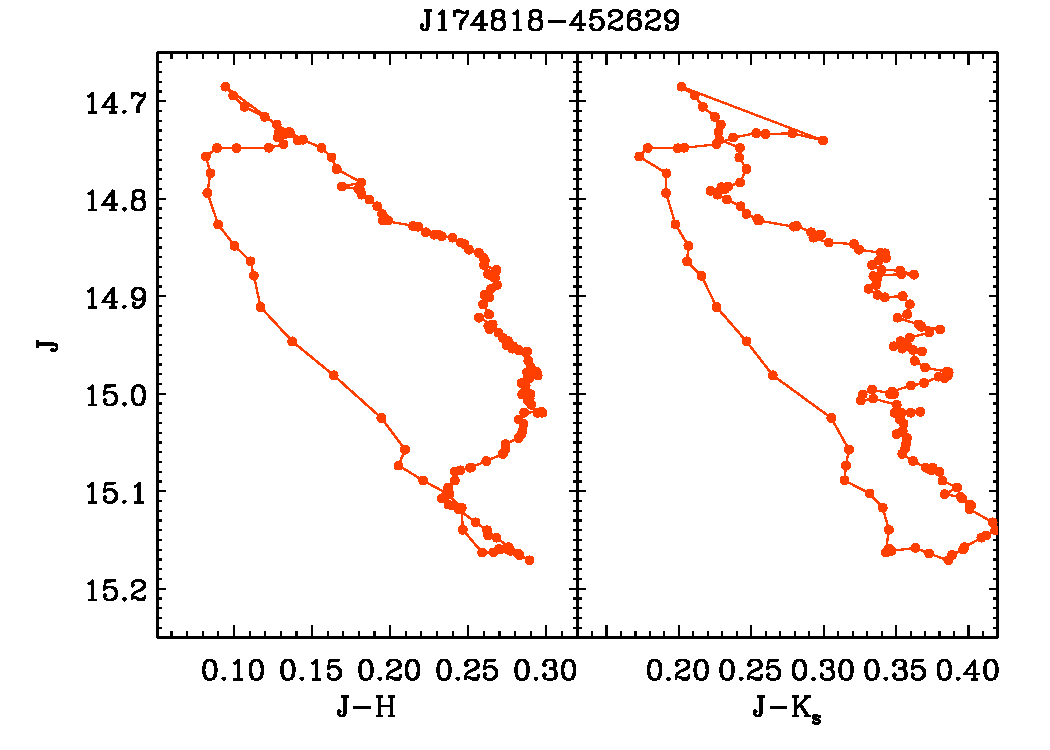
\includegraphics[width=2.0in]{new_plots/rr_cmd_2}\\
%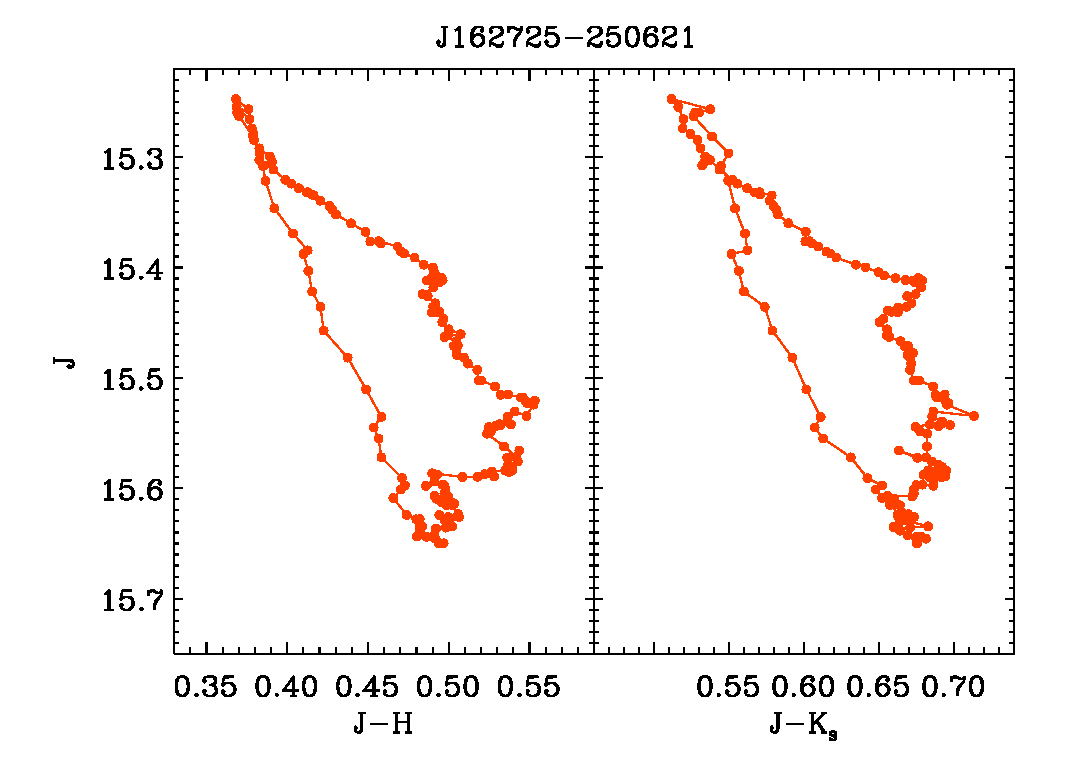
\includegraphics[width=2.0in]{new_plots/rr_cmd_3}
%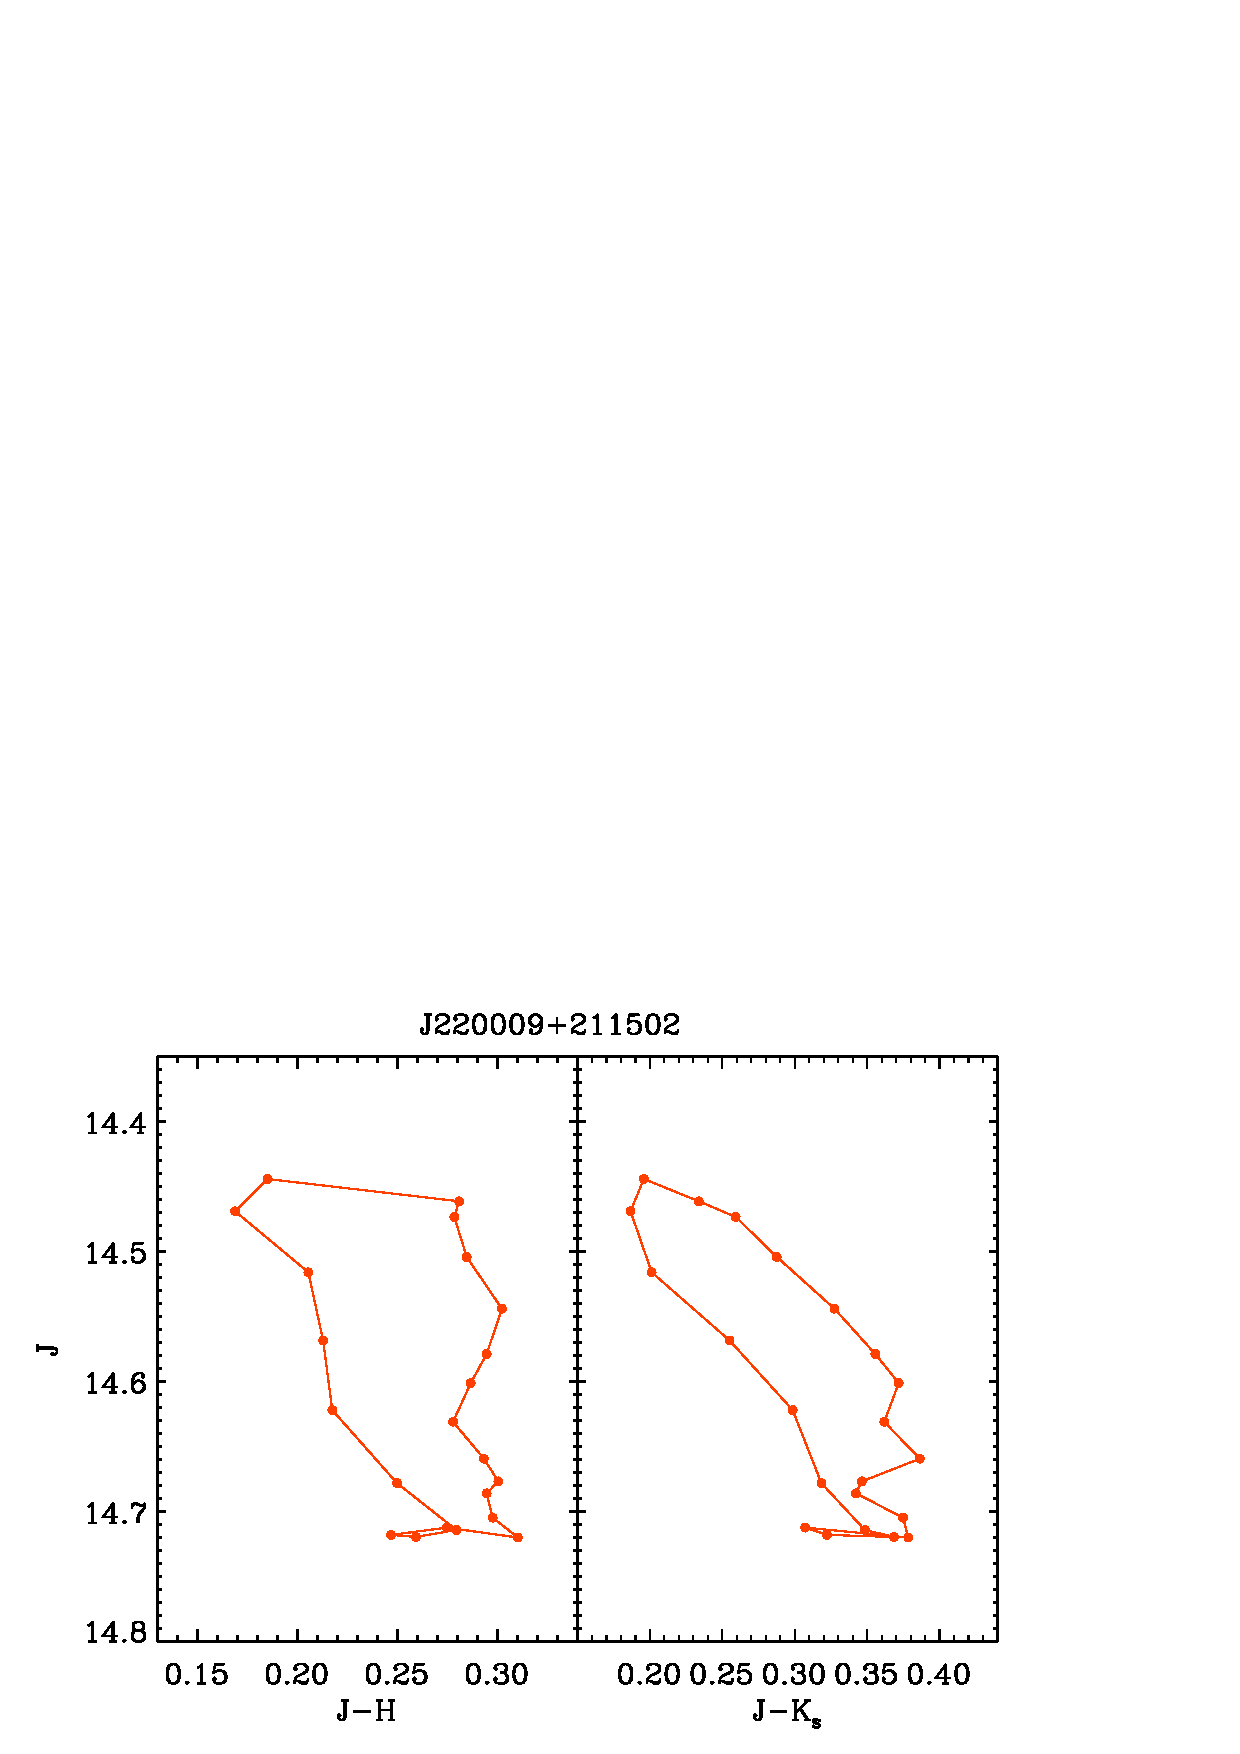
\includegraphics[width=2.0in]{new_plots/rr_cmd_4}
%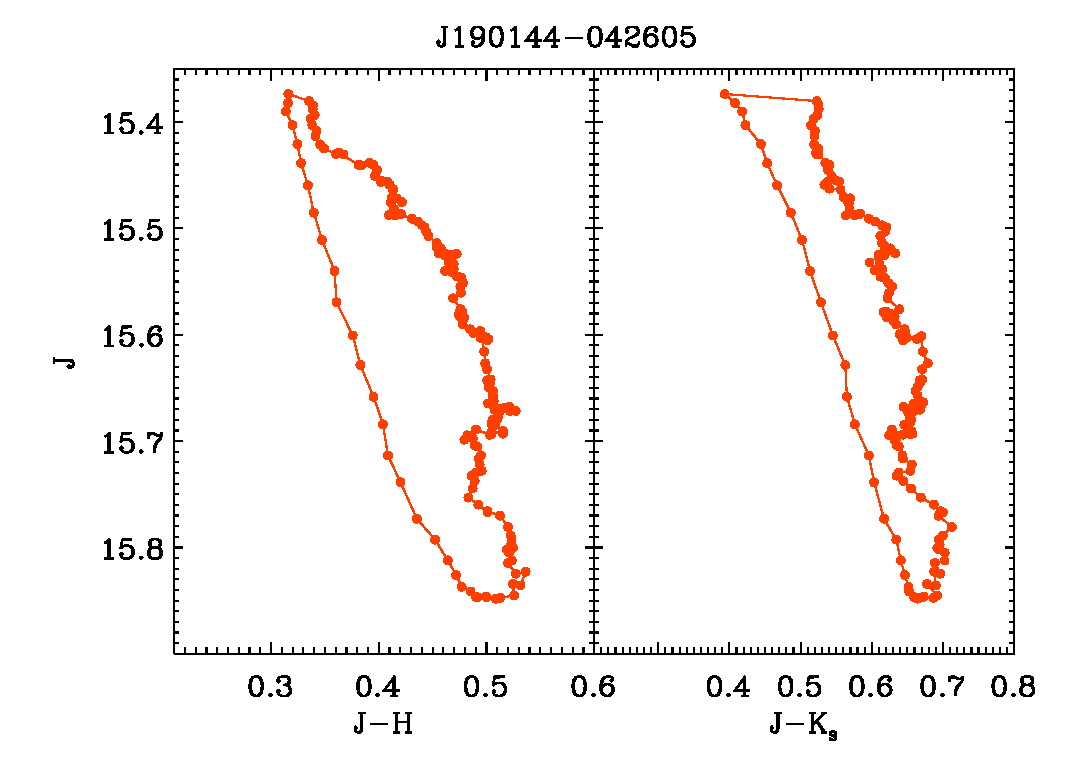
\includegraphics[width=2.0in]{new_plots/rr_cmd_5}\\
%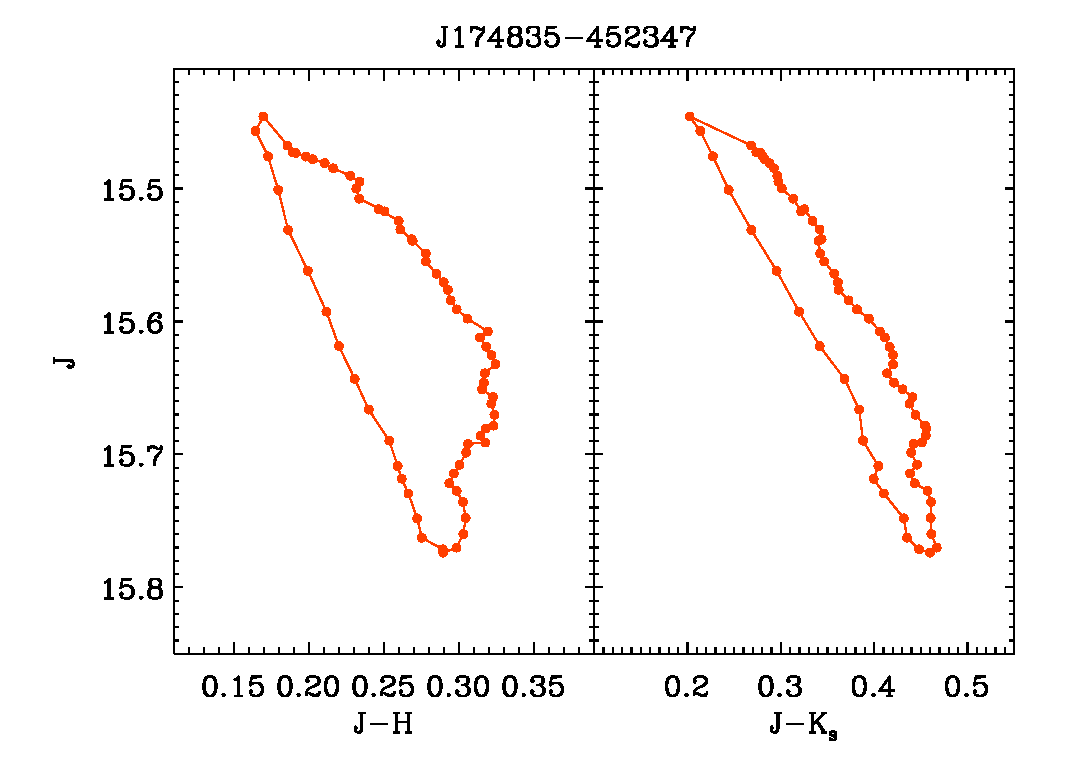
\includegraphics[width=2.0in]{new_plots/rr_cmd_6}
%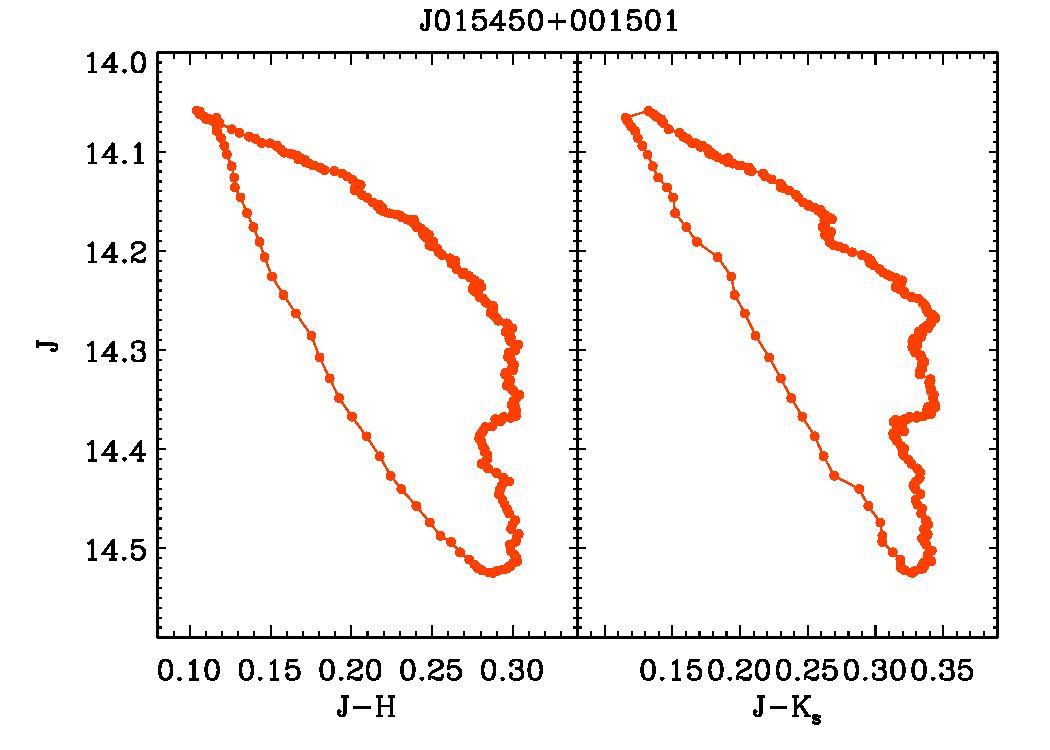
\includegraphics[width=2.0in]{new_plots/rr_cmd_7}
%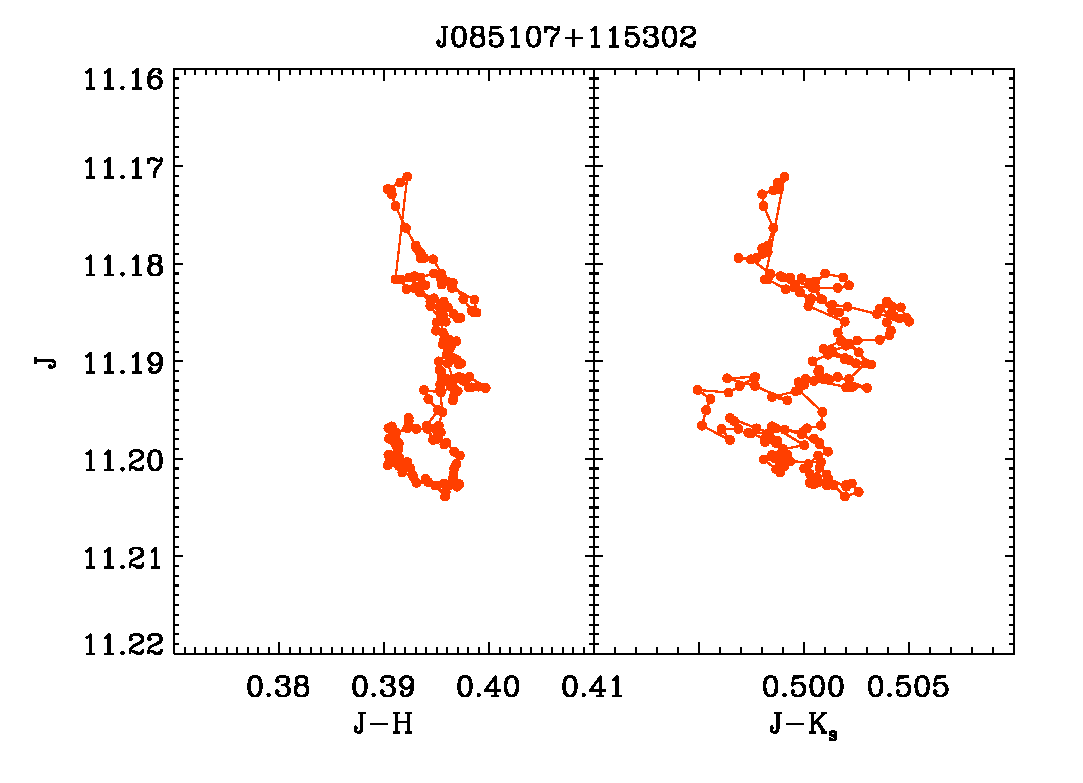
\includegraphics[width=2.0in]{new_plots/rr_cmd_8}

\begin{figure*}[]
\centering
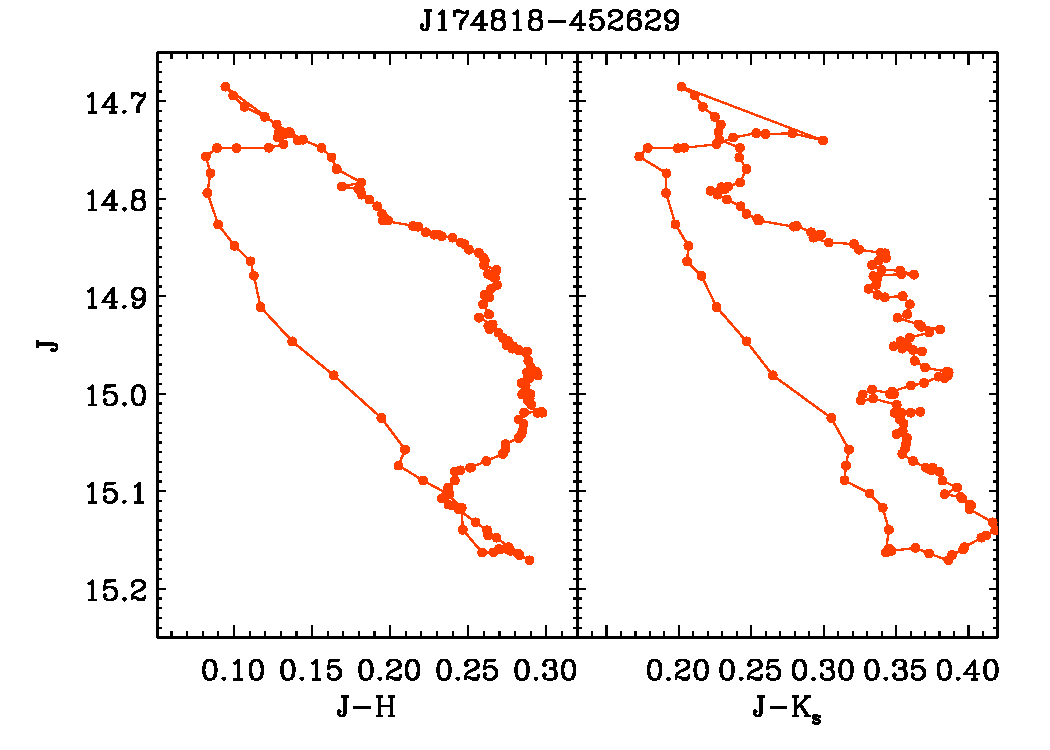
\includegraphics[width=2.0in]{new_plots/rr_cmd_2}
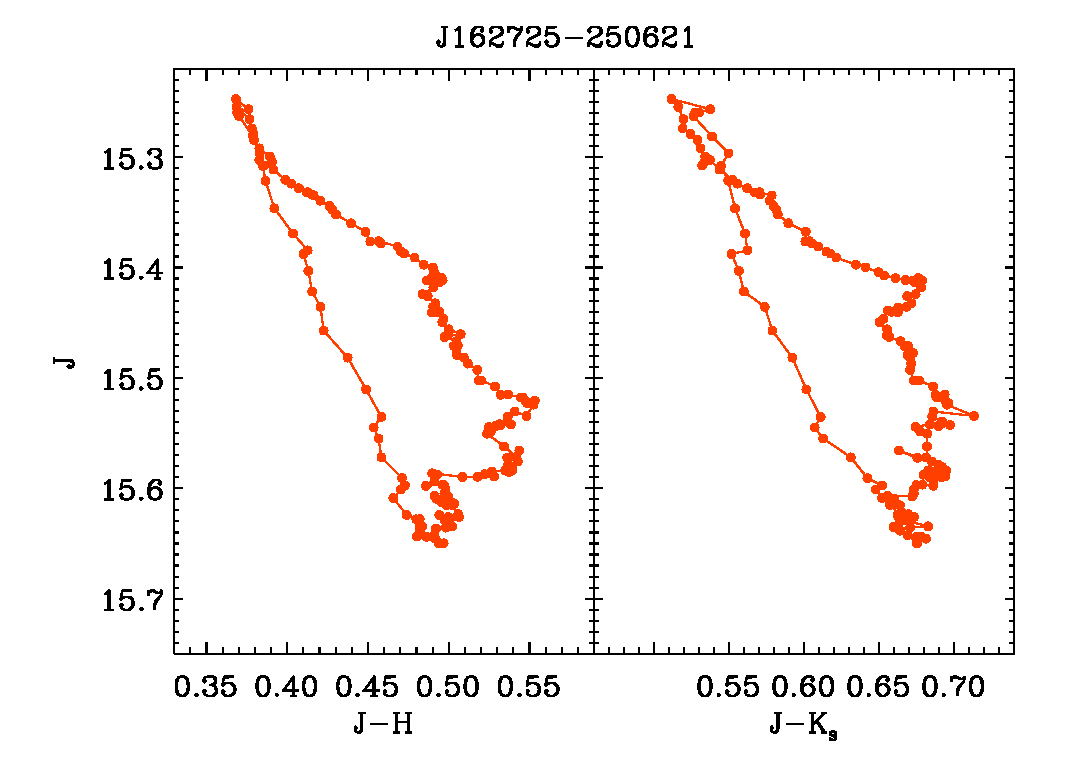
\includegraphics[width=2.0in]{new_plots/rr_cmd_3}
\includegraphics[width=2.0in]{new_plots/rr_cmd_4}\\
\includegraphics[width=2.0in]{new_plots/rr_cmd_5}
\includegraphics[width=2.0in]{new_plots/rr_cmd_6}
\includegraphics[width=2.0in]{new_plots/rr_cmd_7}
\caption{CMD of RRab pulsators}
\label{cmdshort}
\end{figure*}

\begin{figure*}[]
\centering
\includegraphics[width=2.5in]{new_plots/rr_cmd_9}
\includegraphics[width=2.5in]{new_plots/rr_cmd_10}
\caption{CMD of Pulsators (Cepheids)  with periods longer than 2 days}
\label{cmdlong}
\end{figure*}



%%%%%%%%%%%%%%%%%%%%%%%%%
\section{Non-periodic Variables}
Plavchan and student have done lots of work on this for $\rho$ Oph field. We will only add other things that were identified by hand

\begin{deluxetable*}{lccccccccccc}
%\rotate
\setlength{\tabcolsep}{0.02in} 
\tabletypesize{\tiny}
\tablecolumns{11}
\tablecaption{The catalog of quasi-periodic variables. (THIS TEX FILE NEEDS TO BE REVISED TO ONLY INCLUDE THE ACTUALLY INTERESTING OBJECTS, MOST ARE ALREADY SHOWN)}
\tablehead{
	\colhead{ObjectID}&
	\colhead{FieldID} &
	\colhead{RA} &
	\colhead{Dec} &
	\colhead{$\langle J\rangle$} &
	\colhead{$\langle H\rangle$} & 
	\colhead{$\langle K_s\rangle$} &
	\colhead{\# epochs} &
	\colhead{$\sigma_J$} &
	\colhead{$\sigma_H$} &
	\colhead{$\sigma_K$} \\
	\colhead{(hhmmss+ddmmss)}&
	\colhead{} &
	\colhead{(deg)} &
	\colhead{(deg)} &
	\colhead{(mag)} &
	\colhead{(mag)} & 
	\colhead{(mag)} &
	\colhead{} &
	\colhead{(mag)} &
	\colhead{(mag)} &
	\colhead{(mag)}
	}
\startdata
  J162659-243556 &  90009 &   246.74608 &   -24.59911 & 16.40 & 13.45 & 11.86 &   1543 &  0.01401 &  0.00569 &  0.00182 \\
  J162722-244807 &  90009 &   246.84578 &   -24.80195 & 10.92 &  9.83 &  9.34 &   1581 & -0.00000 & -0.00000 &  0.00046 \\
  J162718-245453 &  90009 &   246.82655 &   -24.91494 & 11.42 & 10.54 &  9.95 &   1567 &  0.07128 &  0.04564 &  0.02912 %\\
%  J085113+115140 &  90067 &   132.80576 &    11.86123 & 11.59 & 11.04 & 10.91 &   3692 &  0.00051 &  0.00021 &  0.00008 \\
%  J070115+482309 &  90161 &   105.31503 &    48.38600 & 14.97 & 14.29 & 13.96 &   2576 &  0.00321 &  0.00378 &  0.00257 \\
%  J183935+485234 &  90182 &   279.89651 &    48.87616 & 12.54 & 11.94 & 11.80 &   1703 &  0.00011 &  0.00009 &  0.00001 \\
%  J120151-495519 &  90217 &   180.46277 &   -49.92199 & 15.08 & 14.43 & 14.28 &   1687 &  0.00265 &  0.00226 &  0.00266 \\
%  J145636-444345 &  90273 &   224.15221 &   -44.72928 & 16.45 & 15.87 & 15.41 &   1592 &  0.02448 &  0.00069 & -0.00000 \\
%  J145709-444631 &  90273 &   224.29086 &   -44.77550 &  8.07 &  7.12 &  6.74 &   1780 & -0.00000 & -0.00000 & -0.00000 \\
%  J174802-450540 &  90279 &   267.01227 &   -45.09446 &  9.61 &  8.66 &  8.30 &    961 &  0.00008 & -0.00000 &  0.00001 \\
%  J174805-452207 &  90279 &   267.02106 &   -45.36878 &  9.21 &  8.27 &  7.92 &    970 &  0.00048 & -0.00000 & -0.00000 \\
%  J174815-450235 &  90279 &   267.06516 &   -45.04307 & 10.70 &  9.76 &  9.43 &    975 &  0.00036 &  0.00015 &  0.00023 \\
%  J174827-451826 &  90279 &   267.11459 &   -45.30724 &  9.72 &  8.76 &  8.35 &    978 &  0.00030 & -0.00000 &  0.00043 \\
%  J174838-451704 &  90279 &   267.16211 &   -45.28449 & 10.28 &  9.38 &  9.13 &    977 &  0.00076 &  0.00066 &  0.00077 \\
%  J045901-655830 &  90400 &    74.75442 &   -65.97512 & 13.09 & 11.50 & 10.25 &    377 &  0.03248 &  0.02343 &  0.01467 \\
%  J045923-654151 &  90400 &    74.84740 &   -65.69778 & 11.68 & 11.70 & 11.70 &    378 &  0.00055 &  0.00057 &  0.00082 \\
%  J045929-651532 &  90400 &    74.87146 &   -65.25909 & 11.64 & 11.27 & 11.15 &    378 &  0.00132 &  0.00115 &  0.00081 \\
%  J051429-703352 &  90401 &    78.62468 &   -70.56453 & 13.97 & 13.58 & 13.49 &    156 &  0.00281 &  0.00201 &  0.00236 \\
%  J185106-044436 &  90547 &   282.77625 &    -4.74352 & 14.73 & 13.97 & 13.70 &    656 &  0.00448 &  0.00353 &  0.00138 \\
%  J185103-035333 &  90547 &   282.76584 &    -3.89267 & 14.37 & 13.28 & 12.82 &    658 &  0.00338 &  0.00654 &  0.00344 \\
%  J185107-043809 &  90547 &   282.78073 &    -4.63600 &  9.34 &  8.11 &  7.58 &    657 &  0.00342 &  0.00271 &  0.00316 \\
%  J185105-040211 &  90547 &   282.77246 &    -4.03639 &  8.68 &  7.34 &  6.73 &    657 &  0.00074 & -0.00000 &  0.00030 \\
%  J185107-040741 &  90547 &   282.77966 &    -4.12830 & 11.39 & 10.02 &  9.44 &    671 &  0.00569 &  0.00353 &  0.00877 \\
%  J185110-044206 &  90547 &   282.79578 &    -4.70182 &  9.82 &  8.48 &  7.82 &    659 &  0.00422 &  0.00240 &  0.00228 \\
%  J185111-040919 &  90547 &   282.79929 &    -4.15536 & 10.40 &  8.90 &  8.19 &    671 &  0.00149 &  0.00090 &  0.00079 \\
%  J185115-040308 &  90547 &   282.81610 &    -4.05230 & 10.95 &  9.48 &  8.80 &    655 &  0.00139 &  0.00129 &  0.00113 \\
%  J185117-042032 &  90547 &   282.82101 &    -4.34225 & 10.83 &  9.10 &  8.07 &    341 &  0.04964 &  0.05142 &  0.03403 \\
%  J185119-041940 &  90547 &   282.82953 &    -4.32796 & 12.71 & 10.80 &  9.98 &    671 &  0.00049 &  0.00034 &  0.00021 \\
%  J185118-040122 &  90547 &   282.82547 &    -4.02293 &  6.13 &  5.11 &  4.71 &    659 &  0.00118 &  0.00106 &  0.00027 \\
%  J185117-034801 &  90547 &   282.82455 &    -3.80040 & 14.07 & 13.53 & 13.31 &    626 &  0.01135 &  0.01944 &  0.01341 \\
%  J185120-040910 &  90547 &   282.83423 &    -4.15294 &  9.14 &  7.63 &  6.89 &    671 &  0.00477 &  0.00328 &  0.00314 \\
%  J185122-042540 &  90547 &   282.84491 &    -4.42778 &  9.98 &  8.50 &  7.84 &    671 &  0.00031 & -0.00000 &  0.00025 \\
%  J185123-040901 &  90547 &   282.84732 &    -4.15043 & 11.11 &  9.59 &  8.68 &    671 &  0.08413 &  0.07953 &  0.05669 \\
%  J185126-043722 &  90547 &   282.85895 &    -4.62279 &  9.81 &  8.47 &  7.84 &    659 &  0.00090 &  0.00024 &  0.00031 \\
%  J185128-043730 &  90547 &   282.86917 &    -4.62510 & 10.36 &  9.42 &  9.11 &    659 &  0.00055 &  0.00046 &  0.00022 \\
%  J185131-041152 &  90547 &   282.88177 &    -4.19799 & 11.24 &  9.69 &  9.03 &    670 &  0.00019 &  0.00010 &  0.00000 \\
%  J185131-041008 &  90547 &   282.88171 &    -4.16911 & 11.49 &  9.91 &  9.15 &    667 &  0.00493 &  0.00354 &  0.00280 \\
%  J204114-045934 &  90813 &   310.30966 &    -4.99282 &  5.98 &  5.11 &  4.79 &   1549 &  0.00022 &  0.00035 & -0.00000 \\
%  J190143-041034 &  90808 &   285.43005 &    -4.17615 &  9.89 &  8.78 &  8.32 &   1817 &  0.00197 &  0.00201 &  0.00185 \\
%  J190145-043446 &  90808 &   285.43933 &    -4.57968 &  8.85 &  7.53 &  6.97 &   1868 &  0.00097 &  0.00039 &  0.00069 \\
%  J190150-043108 &  90808 &   285.46085 &    -4.51908 & 10.34 &  9.11 &  8.53 &   1876 &  0.03867 &  0.04312 &  0.03306 \\
%  J190151-040203 &  90808 &   285.46252 &    -4.03425 & 11.49 & 10.39 & 10.04 &   1821 &  0.00176 &  0.00173 &  0.00122 \\
%  J190154-042902 &  90808 &   285.47894 &    -4.48397 & 10.41 &  9.24 &  8.76 &   1877 &  0.00131 &  0.00097 &  0.00092 \\
%  J190155-042229 &  90808 &   285.48291 &    -4.37489 &  8.19 &  7.10 &  6.65 &   1875 &  0.00086 &  0.00033 &  0.00050 \\
%  J190202-041641 &  90808 &   285.51172 &    -4.27820 & 14.25 & 13.39 & 13.19 &   1823 &  0.00100 &  0.00223 &  0.00235 \\
%  J190211-045050 &  90808 &   285.54877 &    -4.84750 & 14.36 & 13.62 & 13.43 &   1764 &  0.00062 &  0.00130 &  0.00163 
\enddata
\label{lltable}
\end{deluxetable*}


\begin{figure}[]
\centering
\includegraphics[width=3.0in]{new_plots/nova}
\caption{LMC, 377 epochs over 90 days, looks kinda like nova of some sort, no other known observations (that i've found)}
\label{nova}
\end{figure}


\begin{figure*}[]
\centering
\includegraphics[width=2.0in]{new_plots/ll_22}
\includegraphics[width=2.0in]{new_plots/ll_23}
\includegraphics[width=2.0in]{new_plots/ll_24}
\includegraphics[width=2.0in]{new_plots/ll_25}
\includegraphics[width=2.0in]{new_plots/ll_26}
\includegraphics[width=2.0in]{new_plots/ll_32}
\includegraphics[width=2.0in]{new_plots/ll_36}
\includegraphics[width=2.0in]{new_plots/ll_40}
\includegraphics[width=2.0in]{new_plots/ll_41}
\caption{some long quasi-periodic variable objects. a couple look like DY Per's maybe? Nothing quite like RCB}
\label{ll}
\end{figure*}




%%%%%%%%%%%%%%%%%%%%%%%%%
%\section{Transient Objects}
% 
% have not been able to recover anything i believe...



%%%%%%%%%%%%%%%%%%%%%%%%%
%\section{Variability Characteristics}
%
%plots about ``color'' of variability, and overall trends

%%%%%%%%%%%%%%%%%%%%%%%%%%%%%
\section{Conclusions}



%%%%%%%%%%%%%%%%%%%%%%%%%
\acknowledgements
The authors acknowledge support from NASA ADP grant NNX09AC77G.

This publication makes use of data products from the Two Micron All Sky Survey, which is a joint project of the University of Massachusetts and the Infrared Processing and Analysis Center/California Institute of Technology, funded by the National Aeronautics and Space Administration and the National Science Foundation.

\begin{deluxetable*}{lccccccccccc}
%\rotate
\setlength{\tabcolsep}{0.02in} 
\tabletypesize{\tiny}
\tablecolumns{12}
\tablecaption{The catalog of binary stars, selected using Fourier modes. The full version of this catalog (146 entries) will be available online.}
\tablehead{
	\colhead{ObjectID}&
	\colhead{FieldID} &
	\colhead{RA} &
	\colhead{Dec} &
	\colhead{Period} &
	\colhead{$\langle J\rangle$} &
	\colhead{$\langle H\rangle$} & 
	\colhead{$\langle K_s\rangle$} &
	\colhead{\# epochs} &
	\colhead{$a_2$} &
	\colhead{$a_4$} &
	\colhead{$b_1$} \\
	\colhead{(hhmmss+ddmmss)}&
	\colhead{} &
	\colhead{(deg)} &
	\colhead{(deg)} &
	\colhead{(days)} &
	\colhead{(mag)} &
	\colhead{(mag)} & 
	\colhead{(mag)} &
	\colhead{} &
	\colhead{} &
	\colhead{} &
	\colhead{}
	}
\startdata
  J015452+011053 &  90004 &    28.72067 &     1.18153 &    0.37205 & 13.62 & 12.94 & 12.72 &   2956 & -0.00098 &  0.00166 &  0.01248 \\
  J015429+005327 &  90004 &    28.62207 &     0.89091 &    2.63902 & 15.51 & 14.84 & 14.65 &   2969 &  0.01922 & -0.00187 &  0.01532 \\
  J162709-243408 &  90009 &   246.78799 &   -24.56892 &    4.83045 & 12.63 & 10.25 &  8.91 &   1580 &  0.03721 & -0.00837 &  0.06224 %\\
%  J162722-241757 &  90009 &   246.84555 &   -24.29924 &   11.07096 & 13.31 & 10.69 &  9.39 &   1579 &  0.00352 & -0.00676 &  0.03822 \\
%  J162712-243449 &  90009 &   246.80058 &   -24.58029 &    2.96770 & 15.72 & 13.13 & 11.53 &   1573 & -0.01958 &  0.00499 &  0.13805 \\
%  J162731-243403 &  90009 &   246.87950 &   -24.56752 &    7.10956 & 13.42 & 11.32 & 10.33 &   1489 &  0.00160 &  0.00225 &  0.01450 \\
%  J162730-244726 &  90009 &   246.87859 &   -24.79075 &    1.24486 & 12.18 & 10.39 &  9.47 &   1541 &  0.00130 & -0.01046 &  0.00895 \\
%  J162732-250618 &  90009 &   246.88409 &   -25.10501 &    5.49339 & 10.50 &  9.59 &  9.26 &    837 &  0.00510 &  0.00031 &  0.01545 \\
%  J055701+002859 &  90013 &    89.25748 &     0.48323 &    1.76140 & 15.44 & 14.96 & 14.80 &   3500 &  0.05262 &  0.00067 &  0.05007 \\
%  J055701+002542 &  90013 &    89.25510 &     0.42848 &    0.28211 &  9.12 &  8.74 &  8.64 &   3509 &  0.00592 &  0.00021 &  0.04776 \\
%  J085128+114927 &  90067 &   132.86740 &    11.82437 &    0.44144 & 11.80 & 11.55 & 11.48 &   3691 & -0.00024 & -0.00966 &  0.04081 \\
%  J085126+115612 &  90067 &   132.86143 &    11.93679 &    0.27089 & 13.80 & 13.22 & 13.10 &   3692 & -0.00104 & -0.00977 &  0.04025 \\
%  J085118+114554 &  90067 &   132.82509 &    11.76513 &   10.33827 & 11.63 & 11.37 & 11.30 &   3692 &  0.00402 & -0.00023 &  0.00492 \\
%  J085120+115326 &  90067 &   132.83675 &    11.89067 &    0.53390 & 10.32 & 10.11 & 10.04 &   3692 &  0.00306 &  0.00814 &  0.00748 \\
%  J085125+120256 &  90067 &   132.85553 &    12.04910 &    2.82194 & 11.65 & 11.09 & 10.94 &   3692 &  0.00017 & -0.00029 & -0.00167 \\
%  J085127+121148 &  90067 &   132.86380 &    12.19690 &    1.23714 & 13.73 & 13.05 & 12.89 &   3045 &  0.00036 &  0.00779 &  0.00120 \\
%  J085104+114557 &  90067 &   132.77023 &    11.76587 &    0.35967 & 12.41 & 12.13 & 12.05 &   3692 &  0.00033 & -0.00227 &  0.03300 \\
%  J062941-594559 &  90121 &    97.42109 &   -59.76661 &    0.25396 & 15.44 & 14.90 & 14.72 &    562 &  0.00254 & -0.00188 &  0.08179 \\
%  J070028+482903 &  90161 &   105.12016 &    48.48439 &    8.73045 & 15.09 & 14.80 & 14.74 &   1735 &  0.01736 & -0.00425 &  0.01837 \\
%  J183911+492412 &  90182 &   279.79877 &    49.40360 &    2.30379 & 10.72 & 10.48 & 10.39 &   1648 & -0.00196 & -0.00897 &  0.02311 \\
%  J183912+484539 &  90182 &   279.80219 &    48.76101 &    0.24732 & 14.90 & 14.35 & 14.22 &   1665 &  0.00330 &  0.00710 &  0.06576 \\
%  J120203-493407 &  90217 &   180.51393 &   -49.56886 &    0.31187 & 14.63 & 14.23 & 14.15 &   1645 &  0.00429 &  0.00102 &  0.06873 \\
%  J120143-495810 &  90217 &   180.43323 &   -49.96949 &    0.26630 & 15.44 & 14.83 & 14.68 &   1625 &  0.07956 & -0.02468 &  0.22997 \\
%  J120154-500449 &  90217 &   180.47661 &   -50.08054 &    0.42650 & 14.75 & 14.29 & 14.19 &   1686 &  0.01237 & -0.00514 &  0.06157 \\
%  J120156-500555 &  90217 &   180.48529 &   -50.09862 &    0.39287 & 15.65 & 14.97 & 14.81 &   1685 &  0.08488 &  0.00642 &  0.13704 \\
%  J120148-500556 &  90217 &   180.45276 &   -50.09896 &    8.86194 & 16.07 & 15.60 & 15.33 &   1686 &  0.00748 &  0.00181 &  0.01856 \\
%  J120204-501930 &  90217 &   180.51930 &   -50.32524 &    0.98914 & 15.62 & 15.09 & 14.96 &   1687 &  0.04565 & -0.01313 &  0.05934 \\
%  J120148-502636 &  90217 &   180.45296 &   -50.44360 &   20.03178 & 12.96 & 12.44 & 12.32 &   1684 &  0.00483 &  0.02787 &  0.01200 \\
%  J203134-491626 &  90234 &   307.89499 &   -49.27414 &    0.37927 & 11.31 & 11.05 & 10.99 &   2073 &  0.01320 &  0.00063 &  0.09909 \\
%  J033147+374651 &  90247 &    52.94954 &    37.78098 &    0.24758 & 15.01 & 14.31 & 14.13 &   1954 &  0.04697 & -0.00304 &  0.19912 \\
%  J033148+372337 &  90247 &    52.95244 &    37.39380 &   11.77838 & 10.29 & 10.09 &  9.97 &   1955 &  0.02439 & -0.00044 &  0.02056 \\
%  J033221+370115 &  90247 &    53.08871 &    37.02101 &    0.97323 & 14.00 & 13.78 & 13.68 &   1961 &  0.06519 & -0.00502 &  0.10921 \\
%  J033155+370312 &  90247 &    52.98239 &    37.05349 &    5.39081 & 14.97 & 14.29 & 14.14 &   1042 &  0.01886 & -0.00063 &  0.01986 \\
%  J145701-443246 &  90273 &   224.25725 &   -44.54613 &    0.39646 & 15.53 & 14.89 & 14.72 &   1778 &  0.01599 & -0.01311 &  0.05365 \\
%  J145655-443458 &  90273 &   224.22940 &   -44.58299 &    4.33012 & 11.29 & 11.03 & 10.97 &   1780 &  0.02749 & -0.00200 &  0.02921 \\
%  J145702-443607 &  90273 &   224.26210 &   -44.60215 &    0.39703 & 15.91 & 15.50 & 15.30 &   1777 &  0.01396 & -0.00751 &  0.11556 \\
%  J145659-445631 &  90273 &   224.24594 &   -44.94199 &    0.45362 & 12.84 & 12.68 & 12.64 &   1779 &  0.02166 & -0.00838 &  0.08787 \\
%  J145635-450743 &  90273 &   224.14778 &   -45.12863 &    2.56014 & 13.96 & 13.33 & 13.17 &   1776 &  0.03220 &  0.00755 &  0.03226 \\
%  J145652-451118 &  90273 &   224.21803 &   -45.18854 &    0.55061 & 14.30 & 14.07 & 14.01 &   1779 & -0.00002 & -0.00602 &  0.03079 \\
%  J145704-451006 &  90273 &   224.26820 &   -45.16841 &    0.26318 & 16.16 & 15.59 & 15.33 &   1750 &  0.01405 & -0.00519 &  0.11364 \\
%  J174803-451052 &  90279 &   267.01480 &   -45.18124 &    0.26071 & 15.74 & 15.13 & 14.99 &    967 &  0.01753 &  0.01239 &  0.14602 \\
%  J174816-450132 &  90279 &   267.06683 &   -45.02557 &    0.47329 & 15.89 & 15.52 & 15.29 &    915 &  0.00655 & -0.01954 &  0.08728 \\
%  J174812-452052 &  90279 &   267.05295 &   -45.34779 &    0.35342 & 15.91 & 15.50 & 15.28 &    977 &  0.02436 & -0.01054 &  0.11879 \\
%  J174816-450721 &  90279 &   267.07056 &   -45.12272 &    2.03495 & 13.69 & 13.36 & 13.24 &    977 &  0.12595 &  0.01339 &  0.17904 \\
%  J174817-450526 &  90279 &   267.07242 &   -45.09068 &    3.30132 & 13.04 & 12.80 & 12.71 &    972 &  0.00006 &  0.00065 &  0.01908 \\
%  J174824-451553 &  90279 &   267.10104 &   -45.26499 &    2.41243 & 15.76 & 15.02 & 14.79 &    955 &  0.02394 &  0.00784 &  0.01810 \\
%  J174822-452656 &  90279 &   267.09485 &   -45.44893 &    0.59503 & 15.51 & 15.23 & 15.13 &    976 &  0.04999 &  0.01303 &  0.14079 \\
%  J174828-450939 &  90279 &   267.11728 &   -45.16095 &    3.72376 & 14.02 & 13.56 & 13.43 &    977 &  0.03455 & -0.00117 &  0.09429 \\
%  J174826-451908 &  90279 &   267.11017 &   -45.31910 &    3.30828 & 14.69 & 14.31 & 14.24 &    977 &  0.01981 & -0.00012 &  0.02713 \\
%  J174827-453158 &  90279 &   267.11514 &   -45.53283 &    1.82694 & 12.91 & 12.59 & 12.51 &    977 &  0.01055 &  0.00484 &  0.01690 \\
%  J174835-451735 &  90279 &   267.14725 &   -45.29323 &    0.30196 & 14.68 & 14.27 & 14.17 &    977 &  0.01892 &  0.00401 &  0.07848 \\
%  J174836-451820 &  90279 &   267.15350 &   -45.30573 &    1.39160 & 15.86 & 15.30 & 15.13 &    976 &  0.03567 &  0.00155 &  0.03132 \\
%  J163130+301523 &  90330 &   247.87547 &    30.25646 &    0.77257 & 13.58 & 13.02 & 12.91 &   1191 &  0.00753 &  0.00377 &  0.01189 \\
%  J045958-661240 &  90400 &    74.99316 &   -66.21133 &    1.50095 & 14.80 & 14.55 & 14.48 &    377 &  0.00961 & -0.02627 &  0.01741 \\
%  J045917-654848 &  90400 &    74.82290 &   -65.81361 &    0.39462 & 13.14 & 12.92 & 12.88 &    378 &  0.03466 &  0.00524 &  0.16013 \\
%  J045913-654412 &  90400 &    74.80653 &   -65.73671 &    3.74381 & 14.72 & 14.83 & 14.87 &    378 &  0.06041 & -0.00601 &  0.15783 \\
%  J185102-043502 &  90547 &   282.76102 &    -4.58415 &   16.47569 & 14.84 & 13.89 & 13.55 &    176 &  0.06117 & -0.02029 &  0.03684 \\
%  J185104-044200 &  90547 &   282.76999 &    -4.70012 &    5.65758 & 14.00 & 13.27 & 13.01 &    650 &  0.04399 &  0.00246 &  0.13502 \\
%  J185101-035125 &  90547 &   282.75659 &    -3.85699 &    1.05272 & 14.79 & 14.26 & 14.11 &    153 &  0.04798 & -0.02334 &  0.08546 \\
%  J185105-043731 &  90547 &   282.77197 &    -4.62531 &    3.14487 & 13.68 & 13.14 & 12.94 &    659 &  0.01556 &  0.00169 &  0.02147 \\
%  J185108-043612 &  90547 &   282.78680 &    -4.60343 &    0.88925 & 14.53 & 13.97 & 13.74 &    659 &  0.02151 &  0.00052 &  0.12323 \\
%  J185109-041207 &  90547 &   282.79028 &    -4.20197 &    0.68815 & 14.93 & 14.20 & 13.88 &    671 &  0.01509 & -0.02160 &  0.05178 \\
%  J185110-042403 &  90547 &   282.79462 &    -4.40094 &    0.49365 & 14.83 & 14.06 & 13.75 &    671 & -0.00105 &  0.00110 &  0.03751 \\
%  J185116-040939 &  90547 &   282.81955 &    -4.16108 &    2.39399 & 14.87 & 14.10 & 13.81 &    671 &  0.04460 &  0.00004 &  0.05528 \\
%  J185116-035706 &  90547 &   282.81760 &    -3.95190 &    0.72210 & 15.10 & 14.43 & 14.20 &    644 &  0.02773 & -0.00201 &  0.03097 \\
%  J185117-041221 &  90547 &   282.82245 &    -4.20589 &    4.06764 & 14.34 & 13.47 & 13.09 &    669 &  0.02737 &  0.00131 &  0.02825 \\
%  J185117-040800 &  90547 &   282.82281 &    -4.13351 &   14.90156 & 12.89 & 11.80 & 11.39 &    671 &  0.00206 &  0.02192 &  0.00956 \\
%  J185118-040340 &  90547 &   282.82559 &    -4.06139 &   12.69497 & 12.65 & 11.79 & 11.49 &    659 & -0.00271 & -0.00046 &  0.05750 \\
%  J185117-035531 &  90547 &   282.82449 &    -3.92536 &    0.78048 & 14.91 & 14.41 & 14.19 &    659 &  0.01565 &  0.00068 &  0.05733 \\
%  J185120-042631 &  90547 &   282.83481 &    -4.44198 &    3.35485 & 14.46 & 13.83 & 13.58 &    670 &  0.08504 & -0.00889 &  0.12640 \\
%  J185120-043217 &  90547 &   282.83679 &    -4.53811 &    0.79457 & 15.19 & 14.66 & 14.40 &    650 &  0.03550 & -0.00171 &  0.15034 \\
%  J185122-040908 &  90547 &   282.84427 &    -4.15236 &    3.91567 & 13.94 & 13.29 & 13.02 &    666 &  0.02903 &  0.00664 &  0.08038 \\
%  J185121-034937 &  90547 &   282.84131 &    -3.82711 &   38.70439 & 14.42 & 13.36 & 12.98 &    659 &  0.11038 & -0.02148 &  0.07806 \\
%  J185123-041301 &  90547 &   282.84875 &    -4.21695 &    2.22002 & 14.91 & 13.57 & 13.03 &    671 &  0.05575 &  0.04070 &  0.12222 \\
%  J185124-035453 &  90547 &   282.85266 &    -3.91481 &    5.41117 & 12.79 & 12.41 & 12.24 &    657 &  0.04102 &  0.00417 &  0.03220 \\
%  J185127-040555 &  90547 &   282.86298 &    -4.09866 &    1.55120 & 14.90 & 14.30 & 13.99 &    663 &  0.02086 & -0.00549 &  0.04779 \\
%  J185129-041240 &  90547 &   282.87210 &    -4.21133 &    1.51980 & 12.75 & 12.19 & 11.91 &    671 &  0.03208 & -0.00537 &  0.05641 \\
%  J185130-043214 &  90547 &   282.87820 &    -4.53748 &    0.32250 & 13.15 & 12.53 & 12.31 &    659 &  0.00198 & -0.00019 &  0.03900 \\
%  J185131-043958 &  90547 &   282.88303 &    -4.66630 &    7.39460 & 15.14 & 14.60 & 14.42 &    658 &  0.02716 & -0.01670 &  0.02509 \\
%  J185130-041454 &  90547 &   282.87653 &    -4.24853 &    0.40695 & 14.39 & 13.35 & 12.86 &    662 &  0.01320 &  0.00100 &  0.06711 \\
%  J185132-034916 &  90547 &   282.88580 &    -3.82130 &    0.52294 & 15.00 & 14.48 & 14.28 &    658 & -0.00146 &  0.00222 &  0.06208 \\
%  J185134-040506 &  90547 &   282.89340 &    -4.08508 &    0.37329 & 15.02 & 14.35 & 14.11 &    613 &  0.05277 & -0.00162 &  0.18707 \\
%  J162633+054552 &  90565 &   246.63757 &     5.76469 &    1.26269 & 12.18 & 11.93 & 11.85 &   3387 &  0.00006 & -0.00330 &  0.01049 \\
%  J162651+061141 &  90565 &   246.71591 &     6.19496 &    0.32872 & 15.37 & 14.87 & 14.77 &   3412 &  0.06914 &  0.00806 &  0.20103 \\
%  J162656+055204 &  90565 &   246.73497 &     5.86782 &    0.33997 & 15.06 & 14.40 & 14.23 &   3387 &  0.04894 &  0.00090 &  0.06889 \\
%  J204108-043727 &  90813 &   310.28653 &    -4.62440 &    0.94155 & 15.23 & 14.92 & 14.82 &   1475 &  0.00341 &  0.00148 &  0.02581 \\
%  J204117-045204 &  90813 &   310.32364 &    -4.86790 &    0.60848 & 11.11 & 10.81 & 10.73 &   1546 &  0.01308 & -0.00121 &  0.03214 \\
%  J150011-010308 &  90868 &   225.04974 &    -1.05241 &    6.52426 & 13.71 & 13.09 & 12.94 &   2018 &  0.00215 &  0.00124 &  0.06067 \\
%  J150028-002605 &  90868 &   225.12082 &    -0.43487 &    4.39749 & 13.59 & 13.16 & 13.07 &   2181 &  0.04569 &  0.00158 &  0.04332 \\
%  J083219-012643 &  92026 &   128.07921 &    -1.44534 &    0.31488 & 14.77 & 14.43 & 14.37 &   2158 &  0.00410 & -0.00165 &  0.06851 \\
%  J112145-125734 &  92397 &   170.43802 &   -12.95955 &    0.90552 & 13.61 & 13.24 & 13.15 &   2019 &  0.03999 &  0.00193 &  0.06570 \\
%  J112150-132341 &  92397 &   170.46217 &   -13.39473 &    4.40027 & 15.38 & 14.72 & 14.52 &   2582 &  0.01141 & -0.00130 &  0.00654 \\
%  J220011+211453 &  92409 &   330.04889 &    21.24808 &    0.38438 & 13.42 & 12.95 & 12.84 &   1139 &  0.03134 & -0.00308 &  0.07868 \\
%  J220040+205642 &  92409 &   330.16809 &    20.94524 &    0.26243 & 12.71 & 12.20 & 12.09 &   1487 &  0.01124 &  0.00463 &  0.08092 \\
%  J220029+204625 &  92409 &   330.12122 &    20.77382 &    2.51465 & 15.02 & 14.49 & 14.36 &   1481 &  0.01444 &  0.00411 &  0.02916 \\
%  J082558-384603 &  90312 &   126.49415 &   -38.76768 &    0.59773 & 15.76 & 15.31 & 15.06 &    896 &  0.03614 &  0.01003 &  0.17048 \\
%  J082543-384403 &  90312 &   126.43131 &   -38.73419 &    0.29027 & 15.81 & 15.17 & 14.96 &   3497 &  0.00033 & -0.00066 &  0.02768 \\
%  J082528-384548 &  90312 &   126.36718 &   -38.76350 &   18.68669 & 13.25 & 12.56 & 12.40 &   3501 &  0.00024 & -0.00147 &  0.01889 \\
%  J082552-385818 &  90312 &   126.46972 &   -38.97186 &    1.24876 & 13.07 & 12.90 & 12.82 &   3501 &  0.00394 & -0.00129 &  0.01029 \\
%  J082539-385923 &  90312 &   126.41338 &   -38.98976 &    0.53633 & 15.93 & 15.27 & 15.01 &   3499 &  0.00989 &  0.00177 &  0.02476 \\
%  J082532-390000 &  90312 &   126.38473 &   -39.00024 &    0.96250 & 15.74 & 15.06 & 14.72 &   3499 &  0.01146 &  0.00024 &  0.03298 \\
%  J082527-385748 &  90312 &   126.36284 &   -38.96343 &    5.11000 & 15.82 & 15.34 & 15.05 &   3500 &  0.01101 &  0.00460 &  0.01041 \\
%  J082537-390206 &  90312 &   126.40490 &   -39.03518 &    3.06898 & 14.35 & 13.56 & 13.32 &   3501 & -0.00016 &  0.01597 &  0.03090 \\
%  J082540-390629 &  90312 &   126.41904 &   -39.10830 &    8.22038 & 13.80 & 13.48 & 13.32 &   3501 &  0.00650 & -0.00006 &  0.00759 \\
%  J082536-390505 &  90312 &   126.40147 &   -39.08482 &    0.72365 & 16.15 & 15.45 & 15.10 &   3469 &  0.01356 & -0.00485 &  0.13541 \\
%  J082531-390419 &  90312 &   126.38301 &   -39.07222 &    2.84523 & 14.87 & 14.48 & 14.28 &   3501 &  0.01180 & -0.00051 &  0.01416 \\
%  J082546-391116 &  90312 &   126.44264 &   -39.18783 &    0.89403 & 13.08 & 12.41 & 12.25 &   3500 &  0.00850 &  0.00084 &  0.02767 \\
%  J082554-391457 &  90312 &   126.47564 &   -39.24939 &    0.32871 & 15.99 & 15.44 & 15.20 &   3490 &  0.00425 & -0.00222 &  0.06758 \\
%  J082554-391517 &  90312 &   126.47711 &   -39.25473 &    2.43811 & 14.53 & 14.17 & 13.99 &   3501 &  0.01124 & -0.00025 &  0.01266 \\
%  J082535-391107 &  90312 &   126.39703 &   -39.18530 &    2.65335 & 15.68 & 15.24 & 15.03 &   3486 &  0.00903 &  0.02177 &  0.01720 \\
%  J082519-390900 &  90312 &   126.33107 &   -39.15003 &    1.53547 & 10.39 & 10.35 & 10.31 &   3501 & -0.00044 & -0.00127 &  0.01314 \\
%  J082553-392325 &  90312 &   126.47486 &   -39.39047 &    0.26524 & 15.84 & 15.19 & 14.97 &   3498 &  0.00813 & -0.00460 &  0.06739 \\
%  J082528-391435 &  90312 &   126.36873 &   -39.24311 &    7.77759 & 12.57 & 12.32 & 12.21 &   3501 &  0.03092 &  0.00069 &  0.03273 \\
%  J082545-393115 &  90312 &   126.44075 &   -39.52098 &    1.05851 & 15.62 & 15.04 & 14.79 &   3500 &  0.01520 & -0.00087 &  0.07467 \\
%  J082538-393154 &  90312 &   126.41068 &   -39.53185 &    1.61730 & 15.26 & 14.78 & 14.53 &   3498 &  0.00983 &  0.00035 &  0.01419 \\
%  J082514-392847 &  90312 &   126.31174 &   -39.47999 &    0.32346 & 15.39 & 14.77 & 14.55 &    776 &  0.01095 & -0.01085 &  0.10325 \\
%  J082514-393054 &  90312 &   126.31014 &   -39.51518 &    1.20954 & 16.10 & 15.24 & 14.89 &    340 &  0.01074 & -0.02365 &  0.08500 \\
%  J190141-045637 &  90808 &   285.42319 &    -4.94387 &    0.39817 & 16.08 & 15.53 & 15.20 &   1534 & -0.00034 & -0.00632 &  0.05902 \\
%  J190140-042413 &  90808 &   285.41794 &    -4.40379 &    4.18274 & 12.68 & 12.00 & 11.78 &   1395 &  0.11325 &  0.00259 &  0.20596 \\
%  J190143-045433 &  90808 &   285.43085 &    -4.90944 &    0.97864 & 11.55 & 11.24 & 11.13 &   1813 &  0.03270 & -0.00016 &  0.16665 \\
%  J190144-044202 &  90808 &   285.43378 &    -4.70069 &   12.90985 & 14.16 & 13.29 & 13.04 &   1826 &  0.00110 &  0.00668 &  0.04911 \\
%  J190141-040200 &  90808 &   285.42249 &    -4.03339 &    3.43732 & 15.66 & 15.18 & 14.98 &   1795 &  0.02557 & -0.00164 &  0.02558 \\
%  J190143-042510 &  90808 &   285.43204 &    -4.41967 &    2.17404 & 12.23 & 11.98 & 11.87 &   1869 &  0.00313 &  0.00129 &  0.00708 \\
%  J190145-043549 &  90808 &   285.44009 &    -4.59714 &    2.30905 & 14.30 & 13.65 & 13.42 &   1870 &  0.01241 &  0.00650 &  0.03905 \\
%  J190150-044845 &  90808 &   285.45868 &    -4.81277 &    1.40386 & 12.79 & 12.48 & 12.36 &   1824 &  0.00272 &  0.00161 &  0.02517 \\
%  J190149-043249 &  90808 &   285.45782 &    -4.54700 &    0.65940 & 14.56 & 14.00 & 13.76 &   1829 &  0.01993 &  0.00051 &  0.11456 \\
%  J190153-045525 &  90808 &   285.47470 &    -4.92373 &    0.36737 & 14.64 & 14.12 & 13.98 &   1780 &  0.06335 & -0.00395 &  0.21865 \\
%  J190151-041948 &  90808 &   285.46271 &    -4.33019 &    0.85618 & 14.67 & 14.20 & 14.04 &   1838 &  0.08188 &  0.00641 &  0.14234 \\
%  J190151-041429 &  90808 &   285.46283 &    -4.24141 &    0.48260 & 13.62 & 13.15 & 13.02 &   1821 &  0.01987 &  0.00415 &  0.08323 \\
%  J190154-041038 &  90808 &   285.47760 &    -4.17736 &    1.43323 & 16.06 & 15.51 & 15.18 &   1544 &  0.01990 & -0.00086 &  0.04596 \\
%  J190203-045117 &  90808 &   285.51340 &    -4.85490 &    3.09222 & 13.20 & 12.78 & 12.66 &   1814 &  0.01414 & -0.00062 &  0.01863 \\
%  J190200-041524 &  90808 &   285.50027 &    -4.25692 &    0.33692 & 15.41 & 14.86 & 14.69 &   1813 &  0.09107 &  0.00474 &  0.26582 \\
%  J190159-041226 &  90808 &   285.49963 &    -4.20729 &    0.51847 & 13.21 & 12.73 & 12.58 &   1798 &  0.05774 &  0.00032 &  0.12558 \\
%  J190201-043008 &  90808 &   285.50717 &    -4.50228 &    0.90880 & 15.44 & 14.85 & 14.61 &   1873 &  0.00967 &  0.00376 &  0.06928 \\
%  J190202-043015 &  90808 &   285.50845 &    -4.50444 &    2.48609 & 15.22 & 14.59 & 14.37 &   1874 &  0.06604 &  0.01311 &  0.12422 \\
%  J190202-043150 &  90808 &   285.50946 &    -4.53057 &    1.48158 & 14.08 & 13.61 & 13.46 &   1871 &  0.08627 &  0.00163 &  0.14172 \\
%  J190204-044835 &  90808 &   285.51746 &    -4.80993 &    1.32424 & 12.71 & 12.35 & 12.24 &   1812 &  0.04888 & -0.00128 &  0.07057 \\
%  J190202-042048 &  90808 &   285.50928 &    -4.34667 &   34.77180 & 10.06 &  9.88 &  9.77 &   1872 &  0.01088 & -0.00643 &  0.01021 \\
%  J190204-043939 &  90808 &   285.51865 &    -4.66097 &    1.09214 & 15.68 & 15.13 & 14.90 &   1854 &  0.03771 & -0.00737 &  0.05440 \\
%  J190204-041111 &  90808 &   285.51886 &    -4.18658 &    4.70381 & 13.10 & 12.42 & 12.21 &   1812 &  0.01535 &  0.01186 &  0.02251 \\
%  J190209-043943 &  90808 &   285.54129 &    -4.66221 &    4.34726 & 13.68 & 13.02 & 12.82 &   1858 &  0.04141 &  0.00168 &  0.07681 \\
%  J190207-040513 &  90808 &   285.52985 &    -4.08704 &    0.45384 & 14.00 & 13.65 & 13.54 &   1812 &  0.00935 &  0.00046 &  0.09085 \\
%  J190213-042412 &  90808 &   285.55496 &    -4.40353 &    0.31077 & 15.48 & 14.61 & 14.27 &    764 & -0.00169 &  0.00199 &  0.06804 \\
%  J042616+032358 &  90191 &    66.56686 &     3.39948 &    1.76639 & 15.60 & 14.91 & 14.63 &   2082 &  0.01586 & -0.00365 &  0.01808 \\
%  J082517-385231 &  90312 &   126.32390 &   -38.87542 &    2.33952 & 15.58 & 15.23 & 15.02 &   3473 &  0.05006 &  0.00147 &  0.05588 \\
%  J082554-390844 &  90312 &   126.47524 &   -39.14561 &    8.09002 & 12.91 & 12.15 & 11.91 &   3501 &  0.06730 &  0.00413 &  0.08523 
\enddata
\label{bbtable}
\end{deluxetable*}

\begin{deluxetable*}{lccccccccccc}
%\rotate
\setlength{\tabcolsep}{0.02in} 
\tabletypesize{\tiny}
\tablecolumns{12}
\tablecaption{The catalog of radial pulsating type periodic variables, selected using Fourier modes.}
\tablehead{
	\colhead{ObjectID}&
	\colhead{FieldID} &
	\colhead{RA} &
	\colhead{Dec} &
	\colhead{Period} &
	\colhead{$\langle J\rangle$} &
	\colhead{$\langle H\rangle$} & 
	\colhead{$\langle K_s\rangle$} &
	\colhead{\# epochs} &
	\colhead{$a_2$} &
	\colhead{$a_4$} &
	\colhead{$b_1$} \\
	\colhead{(hhmmss+ddmmss)}&
	\colhead{} &
	\colhead{(deg)} &
	\colhead{(deg)} &
	\colhead{(days)} &
	\colhead{(mag)} &
	\colhead{(mag)} & 
	\colhead{(mag)} &
	\colhead{} &
	\colhead{} &
	\colhead{} &
	\colhead{}
	}
\startdata
  J120137-494808 &  90217 &   180.40575 &   -49.80240 &    0.08777 & 15.22 & 15.03 & 14.95 &   1685 &  0.03441 & -0.14304 &  0.06262 \\
  J183913+492837 &  90182 &   279.80688 &    49.47710 &    0.37473 & 15.96 & 15.68 & 15.43 &   1682 &  0.01161 & -0.14297 &  0.02263 \\
  J174818-452629 &  90279 &   267.07571 &   -45.44157 &    0.41014 & 14.93 & 14.68 & 14.60 &    977 &  0.00012 & -0.00248 & -0.00028 \\
  J162725-250621 &  90009 &   246.85564 &   -25.10589 &    0.48514 & 15.46 & 14.98 & 14.82 &   1579 & -0.00560 &  0.02069 &  0.00883 \\
  J220009+211502 &  92409 &   330.04028 &    21.25065 &    0.51424 & 14.60 & 14.35 & 14.29 &     41 & -0.00234 & -0.02196 &  0.00994 \\
  J190144-042605 &  90808 &   285.43744 &    -4.43475 &    0.52396 & 15.61 & 15.14 & 14.97 &   1879 & -0.00112 & -0.02633 &  0.00154 \\
  J174835-452347 &  90279 &   267.14786 &   -45.39640 &    0.54504 & 15.63 & 15.35 & 15.22 &    972 &  0.02224 & -0.16258 &  0.03681 \\
  J015450+001501 &  90004 &    28.70900 &     0.25038 &    0.63698 & 14.27 & 14.01 & 13.98 &   2972 &  0.02093 & -0.11219 &  0.05638 \\
  J085107+115302 &  90067 &   132.78021 &    11.88394 &    0.67940 & 11.19 & 10.80 & 10.69 &   3692 &  0.03375 & -0.15717 &  0.04523 \\
  J082535-392008 &  90312 &   126.39848 &   -39.33574 &    3.07471 & 12.57 & 11.66 & 11.28 &   3501 &  0.00012 & -0.06949 &  0.04578 \\
  J174811-455323 &  90279 &   267.04904 &   -45.88993 &    6.45956 & 14.02 & 13.40 & 13.27 &    968 &  0.03683 & -0.14425 &  0.06046 
\enddata
\label{rrtable}
\end{deluxetable*}



\bibliography{refs,/Users/james/research/references}
\end{document}




